\documentclass[11pt,a4paper]{article}
\usepackage[a4paper,margin=24mm]{geometry}
\usepackage[T1]{fontenc}
\usepackage[utf8]{inputenc}
\usepackage{lmodern}
\usepackage{amsmath,amssymb,amsthm,mathrsfs}
\usepackage{graphicx}
\usepackage{booktabs,array,tabularx,multirow}
\usepackage[font=small,labelfont=bf]{caption}
\usepackage{enumitem}
\usepackage{microtype}
\usepackage{xcolor}
\definecolor{linkblue}{rgb}{0,0.15,0.5}
\usepackage[colorlinks=true,linkcolor=linkblue,citecolor=linkblue,urlcolor=linkblue]{hyperref}
\usepackage{url}
\graphicspath{{./}{figs/}{paper03_computational_certification_v23_src/figs/}}
\theoremstyle{plain}
\newtheorem{theorem}{Theorem}[section]
\newtheorem{proposition}[theorem]{Proposition}
\newtheorem{lemma}[theorem]{Lemma}
\newtheorem{corollary}[theorem]{Corollary}
\theoremstyle{definition}
\newtheorem{definition}[theorem]{Definition}
\newtheorem{assumption}[theorem]{Assumption}
\theoremstyle{remark}
\newtheorem{remark}[theorem]{Remark}
\newcommand{\R}{\mathbb{R}}
\newcommand{\N}{\mathbb{N}}
\newcommand{\calI}{\mathcal{I}}
\newcommand{\calH}{\mathcal{H}}
\newcommand{\calP}{\mathcal{P}}
\newcommand{\calV}{\mathcal{V}}
\newcommand{\calK}{\mathcal{K}}
\newcommand{\calF}{\mathcal{F}}
\newcommand{\calM}{\mathcal{M}}
\newcommand{\calS}{\mathscr{S}}
\newcommand{\Pol}{\Pi_{\calI}}
\newcommand{\J}{J_{\calI}(T)}
\newcommand{\Gam}{\Gamma_{\calI}}
\newcommand{\rhoHG}{\rho_{\calH,G}}
\newcommand{\ebar}{\bar{e}}
\newcommand{\tfr}[2]{\tfrac{#1}{#2}}
\newcommand{\dd}{\,\mathrm{d}}
\DeclareMathOperator{\conv}{conv}
\DeclareMathOperator{\rank}{rank}
\DeclareMathOperator{\TV}{TV}
\DeclareMathOperator{\Lift}{Lift}
\DeclareMathOperator{\depth}{depth}
\setlength{\parskip}{2pt}
\emergencystretch=2em
\allowdisplaybreaks

\begin{document}

\title{\textbf{Finite certificates of nonviability under incomplete observation:\\ a continuous-to-finite bridge with exact witnesses}}
\author{Amin Abaee\\[0.3em]
{\small Independent Researcher}\\[0.2em]
{\small ORCID: \href{https://orcid.org/0000-0002-0019-1842}{0000-0002-0019-1842}\quad
\href{mailto:amin_abaee@ut.ac.ir}{amin\_abaee@ut.ac.ir}}}
\date{October 15, 2026}
\maketitle

\begin{abstract}
\noindent
Proving that a safety specification \emph{cannot} be met by any controller is harder under partial observation than under full observation, because the certificate must exclude every measurable, information-adapted policy, and the adversary chooses mode, initial state and disturbance after the policy is announced. Naive discretisation of the control proves only the infeasibility of a held-control subclass. This paper constructs finite, solver-attainable and independently checkable certificates for linear systems whose hidden mode is revealed through an exogenous schedule of history partitions. Approximating the admissible controls from outside by block moments and the adversary from inside by stored labels and scenarios yields a finite linear program whose optimal value is a certified lower bound on the continuous-time safety value and whose certified inflation is an upper bound; every dual-feasible point is a finite obstruction certificate valid against every measurable policy, nonviability is eventually detected along any vanishing refinement sequence, and the value admits an exact atomic dual representation (Sion). Certificate size is governed by information--time rank: positive certificates can be taken with at most $r+1$ labels, a scalar-input construction saturates this bound, and the obstruction depth of the belief is a matching lower bound. On a three-branch delayed-observation instance the certificates are carried exactly: every pair of compatible states is viable and a common blind control is safe, yet the triple is obstructed past the exact delay $7/50$; the finite value obeys the closed law $\rho(\calH)=3/50-\frac14\sum_J|J|^2$ on every aligned mesh, certified by one mesh-independent primal--dual witness pair, and HiGHS reproduces it to $4.2\times10^{-17}$. Read prescriptively, the certificate yields an exact delay hierarchy for sub-beliefs, prices candidate observers through an erosion identity, and brackets the installation time of an early partial observer within $[3/25,(6-\sqrt{29})/5]$. All exact statements are machine-verified in rational arithmetic (63 checks); the solver is a confirmation, never a proof object.
\end{abstract}

\medskip
\noindent\textbf{Keywords:} viability theory; incomplete observation; obstruction certificates; linear programming duality; moment relaxation; delayed observation; exact rational verification; certified computation

\medskip
\noindent\textbf{MSC 2020:} 93B03, 49N05, 90C05, 93C05, 65G20

\section{Introduction}\label{sec:intro}

Viability theory asks whether a controller can keep a system inside a constraint set for as long as required \cite{Aubin1991}. Under full observation the computational side of that question is mature: viability kernels are approximated by backward recursions on grids \cite{SaintPierre1994}, by level-set formulations \cite{MitchellBayenTomlin2005}, and by Lagrangian reachability computations that scale considerably further \cite{Maidens2013}; set invariance has a well-developed convex theory \cite{Blanchini1999}; and the minimax reachability of target tubes under set-membership uncertainty was settled early \cite{BertsekasRhodes1971}. Under \emph{incomplete} observation the sufficiency side is carried by output-feedback conditions and estimation tubes \cite{Veliov1993}, but the necessity side---certificates whose validity \emph{proves} that no admissible controller can keep an information state safe---has lacked a computational bridge. The obstruction calculus of \cite{Abaee2026calc} characterises such certificates in continuous time; what is missing is a finite object, computable by a standard solver and checkable by a third party, that carries the same force.

The difficulty is one of quantifier order. The controller announces a policy adapted to its observation history; the adversary then chooses the hidden mode, the initial state inside its cell, and a measurable disturbance. A certificate of nonviability must therefore cover \emph{every} measurable, information-adapted policy. Discretising the control signal and showing that the resulting finite program is infeasible proves only that no \emph{held} control is safe, which is a strictly weaker statement; the direction of approximation matters, and getting it wrong makes infeasibility-by-discretisation arguments unsound.

\subsection{Contributions}

This paper builds the bridge and the tooling around it, and it does so under an explicit division of labour: the mathematics proves soundness and completeness, the solver computes, and exact rational witnesses---not the solver---certify what is printed.

\begin{enumerate}[leftmargin=1.6em,itemsep=2pt]
\item \textbf{A continuous-to-finite theorem for information states} (Theorem~\ref{thm:bridge}). The admissible controls are approximated from \emph{outside} by their block moments, a relaxation that restricts nothing, and the adversary from \emph{inside} by finitely many stored labels and scenarios. The resulting finite linear program has an optimal value $\rhoHG$ that is a certified lower bound on the continuous-time safety value $\J$, and a certified inflation that is an upper bound:
\[
\rhoHG\;\le\;\J\;\le\;\rhoHG+\max_a\ebar_a+\delta_\beta+Lh_t .
\]
Every dual-feasible point of the program is a finite obstruction certificate valid against every measurable policy; nonviability is detected along every admissible refinement sequence; and the value has an exact atomic dual representation, proved through Sion's minimax theorem on the mixed extension of the label set (Corollary~\ref{cor:dual}).
\item \textbf{Certificate size is a matter of information--time rank, not input dimension} (Section~\ref{sec:size}). Whenever a positive certificate exists, one exists with at most $r+1$ safety labels, $r$ the rank of the finite safety-row matrix; a construction with a \emph{scalar} input produces obstructions whose minimal certificates need arbitrarily many witnesses (Proposition~\ref{prop:rank}); and the \emph{obstruction depth} of a belief---the smallest number of compatible modes whose joint presence is already nonviable---is a matching lower bound (Proposition~\ref{prop:depth}). The Helly-type intuition ``$m+1$ compatible states suffice'' is false for common blind control.
\item \textbf{An instance carried exactly from threshold to solver} (Section~\ref{sec:instance}). On a three-branch delayed-observation instance every pair of compatible states is viable, with explicit pairwise policies, and a common blind control keeps every branch safe throughout the blind window; nevertheless the triple is obstructed past the exact delay $\tau^\ast=7/50$. The finite value obeys the closed law $\rho(\calH)=\tfr{3}{50}-\tfr14\sum_{J\in\calH}|J|^2$ on \emph{every} mesh aligned with the observation time (Proposition~\ref{prop:meshlaw}), certified by one mesh-independent primal--dual witness pair; a dual-simplex solver reproduces it to $4.2\times10^{-17}$ across a refinement campaign, and the smallest certifying program has 39 variables.
\item \textbf{The certificate is prescriptive} (Section~\ref{sec:ladder}). Its weights and facet multipliers decode into the instantaneous shared braking authorities of each sub-belief, an exact delay hierarchy $7/50<(15-\sqrt{183})/6<(10-\sqrt{58})/6$ (Theorem~\ref{thm:pairs}), and an \emph{erosion identity} that prices candidate observers: the same witness loses a computable margin when an information cell is split, the ranking of observers by erosion coincides with the ranking of pairs by delay tolerance, and for an observer installed at an intermediate time the identity brackets the critical installation time within $[3/25,(6-\sqrt{29})/5]$, an interval of width below $3\times10^{-3}$ (Proposition~\ref{prop:observer}).
\item \textbf{Exact verification by construction} (Section~\ref{sec:computation}). Primal and dual witnesses are checked in rational arithmetic; a residual-bounded test makes the certificate robust to enclosed data; the Farkas core is mechanised; and a verification script re-derives all 63 exact statements of the paper.
\end{enumerate}

What is \emph{not} claimed is equally explicit (Section~\ref{sec:related}): the two-sided sandwich idea as such belongs to the reachability literature \cite{Maidens2013}, moment relaxation as such to \cite{Lasserre2001,Parrilo2003,Lasserre2008}, and scenario discretisation as such to \cite{CalafioreCampi2006,CampiGaratti2008}. The novelty lies in assembling these into a certificate that is valid against every measurable information-adapted policy under partial observation, in the rank and depth results, and in the prescriptive reading.

\subsection{Organisation}

Section~\ref{sec:setting} fixes the model, the information structure and the safety value. Section~\ref{sec:certificates} defines finite certificates and states the bridge theorem. Section~\ref{sec:size} treats certificate size. Section~\ref{sec:instance} carries the instance, the mesh law and the solver campaign. Section~\ref{sec:ladder} reads the certificate prescriptively. Section~\ref{sec:extensions} records sound extensions beyond exogenous mode observation. Section~\ref{sec:computation} covers complexity and verification, Section~\ref{sec:related} the related work, and Section~\ref{sec:discussion} concludes. Appendix~\ref{app:bridge} proves the bridge theorem; Appendix~\ref{app:ladder} proves the ladder results. The Supplementary Material (SM) contains the remaining proofs, the derivation of the moduli from primitive data, the complete instance arithmetic, the observer-pricing details, and the verification record.
\section{Setting: dynamics, information, and the safety value}\label{sec:setting}

\subsection{Dynamics and constraints}

A hidden mode $\theta\in\Theta:=\{1,\dots,M\}$ selects a linear system
\begin{equation}\label{eq:dyn}
\dot x(t)=A_\theta(t)x(t)+g_\theta(t)+B_\theta(t)u(t)+E_\theta(t)d(t),\qquad t\in[0,T],
\end{equation}
with $A_\theta,g_\theta,B_\theta,E_\theta$ bounded and piecewise continuous, and $B_\theta,E_\theta$ of bounded variation. The initial set in mode $\theta$ is a nonempty compact polytope $P_\theta\subset\R^n$; the input and disturbance sets are nonempty compact polytopes $U=\{v:Fv\le f\}\subset\R^m$ and $D_\theta\subset\R^p$; safety is the closed polyhedron $\calV=\{x:c_i^\top x\le b_i,\ i=1,\dots,s\}$. The initial information state $B_0=\bigcup_\theta\{\theta\}\times P_\theta$ is assumed initially safe, $P_\theta\subseteq\calV$ for every $\theta$ (otherwise a time-zero certificate suffices). For every admissible measurable pair $(u,d)$ the dynamics admit unique Carath\'eodory solutions. Throughout, $X_\theta(t,s)$ denotes the state-transition matrix of $A_\theta$ and $h_Q(v)=\sup_{q\in Q}v^\top q$ the support function of a set $Q$.

\subsection{Information}

At known times $0=\tau_0<\tau_1<\dots<\tau_R=T$ the controller receives exogenous information about the mode: a refining sequence of \emph{history partitions} $\calP_0\preceq\calP_1\preceq\dots\preceq\calP_{R-1}$ of $\Theta$ (for $r'>r$ every cell of $\calP_{r'}$ lies inside a cell of $\calP_r$), the observation history during $I_r=[\tau_r,\tau_{r+1})$ identifying the cell $C_r(\theta)\in\calP_r$ that contains the true mode. Observations do not depend on $x$, $u$ or $d$; active sensing and endogenous observation branching are outside the exact theorem (Section~\ref{sec:extensions} gives sound extensions). We write $\calI$ for the pair (times, partitions) and call it the information structure.

\subsection{Policies, beliefs, and the kernel}

Policies are deterministic, measurable, nonanticipative and adapted to the observation history. Every such policy is represented exactly by cell signals $u_{r,C}\in L^\infty(I_r;U)$, $C\in\calP_r$, the realised control in mode $\theta$ being $u^\pi_\theta(t)=u_{r,C_r(\theta)}(t)$ on $I_r$. Write $\Pol$ for the set of policies. The robust quantifier order is
\begin{equation}\label{eq:quantifiers}
\exists\,\pi\in\Pol\ \ \forall\,\theta\ \ \forall\,x_0\in P_\theta\ \ \forall\,d\in L^\infty([0,T];D_\theta)\ \ \forall\,t\in[0,T]:\quad x^\pi_{\theta,x_0,d}(t)\in\calV ,
\end{equation}
the adversary selecting mode, initial state and disturbance with knowledge of the announced policy; randomised policies are not included.

\begin{definition}[beliefs and the information-constrained kernel]\label{def:kernel}
A \emph{belief} is a nonempty set $B\subseteq\Theta\times\R^n$ of mode--state possibilities (not a probability distribution). The \emph{information-constrained viability kernel} is the set of beliefs for which \eqref{eq:quantifiers} holds with $B$ in place of $B_0$,
\[
\calK^T_\calI=\bigl\{B:\ \exists\pi\ \forall(\theta,x_0)\in B\ \forall d\ \forall t\ \ x^\pi_{\theta,x_0,d}(t)\in\calV\bigr\}.
\]
$B_0$ is \emph{viable} when $B_0\in\calK^T_\calI$ and \emph{obstructed} (nonviable) otherwise.
\end{definition}

Writing $\Lift(K^T_{\mathrm{full}})=\{B:\varnothing\ne B\subseteq K^T_{\mathrm{full}}\}$ for the belief lifting of the full-information kernel, one has $\calK^T_\calI\subseteq\Lift(K^T_{\mathrm{full}})$, and the inclusion is strict in general: the instance of Section~\ref{sec:instance} has every two-state sub-belief viable while the three-state belief is not. Full-information viability is therefore necessary but not sufficient for the information-constrained question.

\subsection{Adjoint safety rows and the safety value}

A \emph{label} is a triple $a=(\theta,i,t)\in\calS:=\Theta\times\{1,\dots,s\}\times[0,T]$: a mode, a facet, and a time. To each label attach the input kernel and the margin
\begin{align}
k_a(\sigma)&=\mathbf 1_{\{\sigma\le t\}}\,B_\theta(\sigma)^\top X_\theta(t,\sigma)^\top c_i,\label{eq:kernel}\\
\beta_a&=b_i-h_{P_\theta}\!\bigl(X_\theta(t,0)^\top c_i\bigr)-\int_0^t c_i^\top X_\theta(t,\sigma)g_\theta(\sigma)\dd\sigma-\int_0^t h_{D_\theta}\!\bigl(E_\theta(\sigma)^\top X_\theta(t,\sigma)^\top c_i\bigr)\dd\sigma,\label{eq:beta}
\end{align}
and to a policy $\pi$ the row functional $\calF_a(\pi)=\int_0^T k_a(\sigma)^\top u^\pi_\theta(\sigma)\dd\sigma-\beta_a$. The margin $\beta_a$ is the worst-case slack of facet $i$ at time $t$ in mode $\theta$ once the adversary has optimised initial state and disturbance; the kernel is the adjoint of the control's influence on that facet.

\begin{proposition}[robust rows]\label{prop:rows}
A policy $\pi$ satisfies \eqref{eq:quantifiers} on $[0,T]$ if and only if $\calF_a(\pi)\le0$ for every $a\in\calS$.
\end{proposition}

The proof (SM~S1) is the linear solution formula: the initial-state and disturbance maximisations separate from the control term because the control signal in a mode does not depend on $x_0$ or $d$, and for polytopic $D_\theta$ a maximising disturbance can be chosen measurably by a fixed vertex order. Define the \emph{minimax safety violation}
\begin{equation}\label{eq:value}
\J=\min_{\pi\in\Pol}\ \max_{a\in\calS}\ \calF_a(\pi).
\end{equation}

\begin{proposition}[value and nonviability]\label{prop:value}
Under hypothesis \textup{(H1)} of Theorem~\ref{thm:bridge} the minimum in \eqref{eq:value} exists, and $B_0\notin\calK^T_\calI$ if and only if $\J>0$.
\end{proposition}

Existence follows from weak-$\ast$ compactness of the policy space (each factor $L^\infty(I_r;U)$ is weak-$\ast$ closed and bounded because $U$ is a compact convex polytope) and weak-$\ast$ continuity of the affine functionals $\calF_a$; the maximum over labels is attained because $a\mapsto\calF_a(\pi)$ is continuous in $t$ under (H1). The equivalence is the definition of the kernel together with closedness of $\calV$: safety at the margin is viability, so $J=0$ still admits a safe policy and nonviability is the \emph{strict} inequality (SM~S1).

\begin{lemma}[information monotonicity]\label{lem:mono}
Let $\calI'$ refine $\calI$ (observations arrive no later and partitions are no coarser at every time). Then $\calK^T_\calI\subseteq\calK^T_{\calI'}$ and $J_{\calI'}(T)\le\J$.
\end{lemma}

\begin{proof}
Every $\calI$-adapted policy is $\calI'$-adapted: a controller with finer information may ignore it. The minimum in \eqref{eq:value} is therefore taken over a larger set.
\end{proof}

The lemma is elementary but load-bearing: it turns a certificate at one delay into certificates at all larger delays (Theorem~\ref{thm:pairs}) and a viable schedule at one observer installation time into viability at all earlier ones (Proposition~\ref{prop:observer}).
\section{Finite certificates and the continuous-to-finite theorem}\label{sec:certificates}

\subsection{The atomic certificate}

Let $\phi_U(g):=\min_{v\in U}g^\top v=-h_U(-g)$. Choose finitely many labels $a_\ell=(\theta_\ell,i_\ell,t_\ell)$, $\ell=1,\dots,q$, and weights $\lambda\in\Delta_q$ (nonnegative, summing to one). For each information cell $C\in\calP_r$ pool the kernels of the labels whose mode lies in the cell, $g_{r,C}(\sigma)=\sum_{\ell:\theta_\ell\in C}\lambda_\ell k_{a_\ell}(\sigma)$, and define the \emph{certificate margin}
\begin{equation}\label{eq:margin}
\Gam(\lambda,a)=\sum_{r=0}^{R-1}\int_{I_r}\sum_{C\in\calP_r}\phi_U\bigl(g_{r,C}(\sigma)\bigr)\dd\sigma-\sum_{\ell=1}^q\lambda_\ell\beta_{a_\ell}.
\end{equation}
The pooling is where the information structure enters: on an interval during which two modes are indistinguishable, their kernels are summed before the controller's best response is taken, because a single control signal must serve both.

\begin{lemma}[semantics and tightness of the margin]\label{lem:semantics}
For every policy $\pi$, $\sum_\ell\lambda_\ell\calF_{a_\ell}(\pi)\ge\Gam(\lambda,a)$, with equality for the policy that selects, in each cell and at almost every time, a minimising vertex of $v\mapsto g_{r,C}(\sigma)^\top v$ in a fixed vertex order. Consequently, if $\Gam(\lambda,a)>0$ then no admissible information-adapted policy is safe: for every $\pi$ some stored label satisfies $\calF_{a_\ell}(\pi)\ge\Gam(\lambda,a)>0$, i.e.\ an admissible realisation violates facet $i_\ell$ at time $t_\ell$ by at least $\Gam$.
\end{lemma}

The violating label may depend on the policy; the finite list and its weights do not. A positive margin is thus a finite, policy-independent set of adversarial tests combined by an adjoint identity---not an adversarial tree. The proof is in SM~S1.

\subsection{Outer moments, inner adversary, and the finite program}

\paragraph{Outer control moments.}
Choose a control mesh $\calH=\{J_1,\dots,J_H\}$ of $[0,T]$ containing every sensing time, so that each block $J_j$ lies in one observation interval $I_{r(j)}$. Introduce one vector $v_{j,C}\in U$ for every cell $C\in\calP_{r(j)}$ active during $J_j$; $Q=\sum_j|\calP_{r(j)}|$ is the number of information--time blocks. For a label $a$ define the finite row $A_{a,j,C}=\mathbf 1_{\{\theta\in C\}}\int_{J_j}k_a(\sigma)\dd\sigma$, the block average $\bar k_{a,\calH}=|J_j|^{-1}\int_{J_j}k_a$ on $J_j$, and the \emph{moment error}
\begin{equation}\label{eq:momerr}
e_{a,\calH}=\int_0^T h_U\bigl(\bar k_{a,\calH}(\sigma)-k_a(\sigma)\bigr)\dd\sigma,
\end{equation}
for which any verified upper bound $\ebar_a\ge e_{a,\calH}$ may be used. For every measurable policy the block averages of its cell signals belong to $U$ (convexity), and
\begin{equation}\label{eq:outer}
\sum_{j,C}A_{a,j,C}^\top v_{j,C}-\int_0^T k_a(\sigma)^\top u^\pi_{\theta(a)}(\sigma)\dd\sigma\;\le\;\ebar_a .
\end{equation}
Inequality \eqref{eq:outer} is the crucial orientation: \emph{finite feasibility is a necessary condition for continuous-time safety}. The moments do not restrict the real controller to held inputs; they relax it. For a policy held constant on the blocks the averaging term vanishes identically, but the program remains a relaxation even then, because the error bounds are charged to every row (the instance makes this concrete: the held witness policy attains the continuous value $3/50$ while the program returns $3/50-Th/4$).

\paragraph{Inner adversarial approximation.}
On the right-hand side one may use $\beta^+_a\ge\beta_a$ obtained from an explicit admissible initial state and disturbance rather than from exact worst-case optimisation. If $0\le\beta^+_a-\beta_a\le\delta_\beta$ uniformly over the labels used, the approximation is \emph{safe for nonviability}: it weakens the adversary and enlarges the feasible controller set. For instance, with $w_a(\sigma)=\mathbf 1_{\{\sigma\le t\}}E_\theta(\sigma)^\top X_\theta(t,\sigma)^\top c_i$, a piecewise-constant disturbance choosing $d_{a,J}\in\arg\max_{d\in D_\theta}(\int_Jw_a)^\top d$ on a disturbance mesh of width $h_d$ satisfies
\begin{equation}\label{eq:distbound}
0\le\beta^+_a-\beta_a\le R_DV_Dh_d
\end{equation}
when $D_\theta$ has radius $R_D$ about a fixed centre and $\TV(w_a)\le V_D$; the general budget is $\delta_\beta=\delta_{\mathrm{init}}+\delta_{\mathrm{dist}}+\delta_{\mathrm{num}}$ for separately accounted initial-state, disturbance and numerical errors.

\paragraph{The finite program.}
Let $G\subset[0,T]$ be a finite time grid containing $0$, $T$ and every observation time, with covering radius $h_t=\sup_{t}\min_{\hat t\in G}|t-\hat t|$, and let $\calS_G=\Theta\times\{1,\dots,s\}\times G$. Solve
\begin{equation}\label{eq:lp}
\rhoHG=\min_{v,\rho}\ \rho\quad\text{s.t.}\quad A_av-\beta^+_a-\ebar_a\le\rho\ \ (a\in\calS_G),\qquad v_{j,C}\in U .
\end{equation}
The level $\rho$ is an unrestricted real variable; negative values record strict safety slack. The program has $mQ+1$ variables and at most $Ms\,|G|+p_UQ$ inequalities, $p_U$ the number of facets of $U$.

\subsection{The theorem}

\begin{theorem}[continuous-to-finite]\label{thm:bridge}
Assume
\begin{enumerate}[label=\textup{(H\arabic*)},leftmargin=3em,itemsep=1pt]
\item uniformly over policies, modes and facets, $|\calF_{\theta,i,t}(\pi)-\calF_{\theta,i,t'}(\pi)|\le L|t-t'|$;
\item the input kernels satisfy $\TV(k_a)\le V_U$;
\item the label maps $a\mapsto k_a$ (in $L^1$) and $a\mapsto\beta_a$ are continuous on the compact label set $\calS$;
\item $U$ has radius $R_U$ about some fixed centre;
\item the time grid has covering radius at most $h_t$ and the control mesh has maximum block length $h_u$;
\item the stored adversarial data satisfy $0\le\beta^+_a-\beta_a\le\delta_\beta$ for every label used.
\end{enumerate}
Then:
\begin{enumerate}[label=\textup{(\roman*)},leftmargin=2.4em,itemsep=2pt]
\item \textup{(Certified value sandwich.)}
\begin{equation}\label{eq:sandwich}
\rhoHG\;\le\;\J\;\le\;\rhoHG+\max_{a\in\calS_G}\ebar_a+\delta_\beta+Lh_t .
\end{equation}
The uniform choice $\ebar_a\equiv R_UV_Uh_u$ is valid under \textup{(H2), (H4)} and gives the announced special case; the $\max_a\ebar_a$ form is the one that must be used when a looser verified bound was fed to the program.
\item \textup{(Sound finite certificates.)} If $\rhoHG>0$, the dual of \eqref{eq:lp} supplies a finite certificate of nonviability of the continuous-time system, covering every measurable information-adapted policy.
\item \textup{(Completeness under refinement.)} If $B_0\notin\calK^T_\calI$, then along every admissible refinement sequence with $h_u,h_d,h_t\to0$ and stored-scenario widths $\delta_{\mathrm{init}},\delta_{\mathrm{num}}\to0$, the programs eventually return a positive certificate. With exactly stored scenarios, a schedule with block, disturbance and grid widths at most $h$ halts with margin at least $\gamma/2$ as soon as $(R_UV_U+R_DV_D+L)\,h<\gamma/2$, where $\gamma=\J>0$.
\item \textup{(Exact atomic dual representation.)}
\begin{equation}\label{eq:atomic}
\J=\sup\bigl\{\Gam(\lambda,a):\ q\in\N,\ a_1,\dots,a_q\in\calS,\ \lambda\in\Delta_q\bigr\}.
\end{equation}
In particular, nonviability is equivalent to the existence of a positive finite atomic certificate.
\item \textup{(Sparse witnesses.)} Let $r$ be the rank of the safety-row coefficient matrix of \eqref{eq:lp} (the rows $A_a$, excluding the $\rho$-column and the actuator inequalities). Whenever $\rhoHG>0$, a positive certificate exists using at most $r+1\le mQ+1$ safety labels, and it can retain any prescribed margin strictly below $\rhoHG$. If the lifted continuous-time kernels span a space of dimension $r_\calI$, a continuous-time obstruction admits a certificate with at most $r_\calI+1$ labels.
\end{enumerate}
\end{theorem}

The proof is given in Appendix~\ref{app:bridge}; the moduli $L$, $V_U$, $V_D$ and the $L^1$ label-continuity modulus are computed from the primitive data of \eqref{eq:dyn} in SM~S2, so that (H1)--(H3) are not free assumptions.

\begin{corollary}[complete dual calculus]\label{cor:dual}
Under the hypotheses of Theorem~\ref{thm:bridge}:
\textup{(a)} every pair $(\lambda,a)$ satisfies $\Gam(\lambda,a)\le\J\le\max_a\calF_a(\pi)$ for every policy $\pi$;
\textup{(b)} $\J$ is the supremum of $\Gam$ over finite atomic pairs; the supremum over all probability measures on $\calS$ is attained, and attainment by an atomic maximiser is an instance-level fact (three atoms attain it in Section~\ref{sec:instance}), not a general claim;
\textup{(c)} $B_0\notin\calK^T_\calI$ if and only if some finite atomic pair has $\Gam(\lambda,a)>0$; every such pair obstructs every measurable information-adapted policy, and every obstruction arises in this way.
\end{corollary}

The duals therefore form a \emph{complete} certificate system for the class: positivity is the only decision, and the finite program of \eqref{eq:lp} is a mechanical way of searching for a positive pair at a prescribed resolution.

\subsection{The asymmetry at the core of the proof}

Two directions carry the sandwich and they are not symmetric. \emph{Averaging arbitrary controls proves the lower bound}: the block moments of any admissible policy are feasible for \eqref{eq:lp} at objective $\max_a\calF_a(\pi)$, so the relaxed minimum cannot exceed the continuous value. \emph{Implementing piecewise-constant controls proves the upper bound}: the held control read off an optimiser of \eqref{eq:lp} attains its finite rows exactly, and its exit from the continuous value is charged by the error bounds the program actually used, the stored-scenario error, and the grid interpolation error $Lh_t$. Confusing the two directions---using a discretised controller class to prove \emph{infeasibility}---is what makes naive arguments unsound; the finite program is sound for nonviability precisely because its controller class is an outer relaxation while its adversarial tests are genuinely admissible scenarios.
\section{How large is a certificate?}\label{sec:size}

Theorem~\ref{thm:bridge}(v) bounds the support of a positive certificate by $r+1$, where $r$ is the rank of the finite safety-row matrix in the information--time product. The natural question is whether something smaller---the instantaneous input dimension $m$---would do. It does not.

\begin{proposition}[arbitrarily large minimal obstructions with one input]\label{prop:rank}
For every integer $q\ge1$ there is a continuous-time system with scalar input $u(t)\in[0,1]$ and $q+1$ indistinguishable modes such that every proper sub-belief is viable, the full $(q{+}1)$-mode belief is not, and every obstruction certificate involves all $q+1$ modes.
\end{proposition}

\begin{proof}
Let $T=q$ and $I_j=[j-1,j]$. Mode $j\le q$ carries the scalar state $\dot x=\mathbf 1_{I_j}(t)(u-1)$, $x(0)=0$; mode $q+1$ carries $\dot x=-u$, $x(0)=q-\varepsilon$ with $0<\varepsilon<1$. Require $0\le x\le q$ (the terminal bounds are the binding ones, each $x$ being monotone along its mode) and let there be no observations. With $w_j=\int_{I_j}u$, safety requires $w_j\ge1$ for $j\le q$ and $\sum_jw_j\le q-\varepsilon$; summing gives $0\le-\varepsilon$, a contradiction. If mode $q+1$ is removed, $u\equiv1$ is safe; if mode $j\le q$ is removed, $u=0$ on $I_j$ and $u=1$ elsewhere is safe. A certificate supported on fewer than $q+1$ modes would certify the corresponding proper sub-belief (Proposition~\ref{prop:depth} below), contradicting its viability. Equal weights give margin $\varepsilon/(q+1)$; the kernel rank is $q$, so $q+1$ witnesses are necessary and the bound of Theorem~\ref{thm:bridge}(v) is saturated.
\end{proof}

The bound $r+1$ is an upper bound. The following elementary observation supplies the matching lower bound and explains why, on a concrete instance, the realised support can be far below $r+1$.

\begin{definition}[obstruction depth]\label{def:depth}
For a belief $B$ with mode set $\Theta_B$, the \emph{obstruction depth} is
$\depth_\calI(B)=\min\{|\Theta'|:\ \Theta'\subseteq\Theta_B,\ B|_{\Theta'}\notin\calK^T_\calI\}$, the smallest number of compatible modes whose joint presence is already nonviable ($+\infty$ if $B$ is viable). Here $B|_{\Theta'}$ is $B$ restricted to the modes in $\Theta'$, with the induced information structure.
\end{definition}

\begin{proposition}[two-sided support bounds]\label{prop:depth}
Let $(\lambda,a)$ be a positive certificate for $B$ and let $\Theta_\lambda$ be the set of modes carrying positive weight. Then $(\lambda,a)$ is a positive certificate for $B|_{\Theta_\lambda}$, so $|\Theta_\lambda|\ge\depth_\calI(B)$. Consequently every positive certificate uses at least $\depth_\calI(B)$ labels, and under the hypotheses of Theorem~\ref{thm:bridge}
\[
\depth_\calI(B)\;\le\;\min\{q:\ \Gam(\lambda,a)>0\text{ for some }(\lambda,a)\text{ with }q\text{ labels}\}\;\le\;r+1 .
\]
\end{proposition}

\begin{proof}
Restricting the belief to $\Theta_\lambda$ intersects every information cell with $\Theta_\lambda$; the pooled kernels $g_{r,C}$ of the labels with positive weight are unchanged, cells that lose all weight contribute $\phi_U(0)=0$ before and after, and the margins $\beta_{a_\ell}$ are unchanged. Hence $\Gam$ computed for $B|_{\Theta_\lambda}$ equals $\Gam$ computed for $B$, which is positive, and Lemma~\ref{lem:semantics} makes $B|_{\Theta_\lambda}$ nonviable. Each mode in $\Theta_\lambda$ carries at least one label. The upper bound is Theorem~\ref{thm:bridge}(v).
\end{proof}

In the construction of Proposition~\ref{prop:rank} both bounds coincide ($\depth=q+1=r+1$). On the instance of Section~\ref{sec:instance} they do not: at the audited delay the safety-row matrix has full column rank $r=64$, so Theorem~\ref{thm:bridge}(v) allows 65 labels, while the depth is $3$ (every pair is viable) and the exhibited certificate uses exactly three labels. The support of a certificate is governed by the belief's conflict structure, which both bounds measure in the information--time product.

\begin{remark}[why Helly's theorem does not apply]\label{rem:helly}
A statement such as ``at most $m+1$ compatible states suffice to witness nonviability'' is Helly's theorem \cite{Helly1923} for convex common-action sets in $\R^m$. It is valid when the decision is a single vector and false for a common blind control \emph{function}: Proposition~\ref{prop:rank} has $m=1$ and needs $q+1$ witnesses. The correct dimension counts independent temporal and informational control decisions---the rank $r$ of Theorem~\ref{thm:bridge}(v)---and the distinction is consequential for review intervals, delayed sensing and any certificate-size claim; its discrete counterpart is a scoping caveat of the finite audits in \cite{Abaee2026worked}.
\end{remark}
\section{A three-branch delayed-observation instance carried exactly}\label{sec:instance}

The instance is chosen so that every quantity---threshold, policies, certificate, finite program, witnesses---is an exact rational (or quadratic-irrational) number, and so that the three standard tests that are \emph{not} sufficient for the information-constrained question all pass: full-information viability, blind-window safety, and pairwise viability.

\subsection{Plant and exact delay threshold}

Consider the planar double integrator $\dot p=v$, $\dot v=u$ with unit vectors $n_1=(1,0)$, $n_2=(-\tfr35,\tfr45)$, $n_3=(-\tfr35,-\tfr45)$ (so $n_1^\top n_2=n_1^\top n_3=-\tfr35$ and $n_2^\top n_3=-\tfr7{25}$), the hexagonal input set
\[
U=\conv\{\pm n_1,\pm n_2,\pm n_3\}=\{u:\ |u_2|\le\tfr45,\ |2u_1+u_2|\le2,\ |2u_1-u_2|\le2\},
\]
safety $n_i^\top p\le2$ ($i=1,2,3$) and $|v_1|,|v_2|\le\tfr65$ (seven facets, $s=7$), three possible initial states $p_j(0)=\tfr{34}{25}n_j$, $v_j(0)=n_j$ (mode $j$ heads along $n_j$ at unit speed), no disturbance, and the mode unobserved until time $\tau$, when it is revealed exactly. The horizon is $T=\tau+1$ unless stated otherwise. Write $\zeta_j(t)=n_j^\top p_j(t)$ for the critical coordinate of branch $j$.

Under full information the instance is comfortably viable: $u=-n_j$ for one second and then $u=0$ holds $\zeta_j$ at $\tfr{34}{25}+\tfr12=\tfr{93}{50}<2$, with $\|v\|_\infty\le1<\tfr65$ throughout and the noncritical facets negative along the $n_j$-ray.

\begin{proposition}[exact delay threshold of the triple]\label{prop:triple}
For $T\ge\tau+1$, $\J=\tau-\tfr7{50}$. In particular the three-branch belief is viable if and only if $\tau\le\tau^\ast:=\tfr7{50}$.
\end{proposition}

\begin{proof}
\emph{Certificate.} Take one label per branch on its own position facet at $t_\ast=\tau+1$, with kernels $k_j(s)=\mathbf 1_{\{s\le t_\ast\}}(t_\ast-s)n_j$, margins $\beta_j=\tfr{16}{25}-t_\ast$, and weights $\lambda=(\tfr38,\tfr5{16},\tfr5{16})$, which satisfy $\sum_j\lambda_j=1$ and $\sum_j\lambda_jn_j=0$. Before observation the pooled kernel vanishes identically; after observation each mode has its own cell and $\phi_U(\lambda_j(t_\ast-s)n_j)=-\lambda_j(t_\ast-s)$ because $h_U(\pm n_j)=1$. Hence
\begin{equation}\label{eq:gamma-tau}
\Gamma(\tau)=-\int_\tau^{\tau+1}(\tau+1-s)\dd s-\Bigl(\tfr{16}{25}-\tau-1\Bigr)=\tau-\tfr7{50},
\end{equation}
so $\Gamma(\tau)\le\J$ by Lemma~\ref{lem:semantics}. \emph{Policy.} Holding $u=0$ until $\tau$ and braking with $u=-n_j$ for one second afterwards keeps $\zeta_j\le\tfr{34}{25}+\tau+\tfr12$ and every other facet strictly satisfied, so every row value is at most $\tau-\tfr7{50}$ and $\J\le\tau-\tfr7{50}$. Equality at $\tau=\tfr7{50}$ is viable because $\calV$ is closed.
\end{proof}

\subsection{Pairs are viable, and the blind-window exit test misses}

Fix $\tau=\tfr15$ and $T=\tfr65$, where $\Gamma=\tfr3{50}>0$. The common control $u=0$ keeps all three branches safe throughout the blind window ($\zeta_j(\tfr15)=\tfr{39}{25}<2$): the obstruction is \emph{not} that information arrives after an unavoidable physical exit. Nor is it visible pairwise.

\begin{proposition}[pairwise viability at $\tau=1/5$]\label{prop:pairs}
At $\tau=\tfr15$, $T=\tfr65$, every two-mode sub-belief is viable:
\begin{enumerate}[label=\textup{(\alph*)},leftmargin=2.2em,itemsep=1pt]
\item for $\{1,2\}$ (and $\{1,3\}$ by the reflection $v_2\mapsto-v_2$): brake through the blind window with the common control $u=-(n_1+n_2)=(-\tfr25,-\tfr45)\in U$, which decelerates both branches along their normals at rate $\tfr25$, then brake each branch along its own normal to rest; the critical coordinate peaks at $\tfr{2469}{1250}=\tfr{12345}{6250}=1.9752$ on both branches, slack $\tfr{31}{1250}$;
\item for $\{2,3\}$: hold $u=n_1$ through the blind window (both branches decelerate at rate $\tfr35$), then brake each branch along its own normal; the peak is $\tfr{2419}{1250}=1.9352$, slack $\tfr{81}{1250}$.
\end{enumerate}
All seven facets hold at every time on every in-belief branch; the velocity components stay within $1$ (resp.\ $\tfr45$), strictly below $\tfr65$.
\end{proposition}

The proof is a closed-form computation (SM~S3): the window exit velocities are $\tfr{23}{25}$ and $\tfr{22}{25}$, braking to rest adds half their squares. Two tempting variants fail and are shown in Figure~\ref{fig:traj}: holding $u=0$ through the blind window and braking fully afterwards peaks at $\tfr{103}{50}>2$, and inserting a $-\tfr35n_j$ leg after $\tau$ in $\{2,3\}$ peaks at $\tfr{2501}{1250}>2$ at $t=\tfr{29}{25}$. The blind control $u=n_1$ of the pair $\{2,3\}$ drives the \emph{off-belief} branch~1 to $|v_1|=\tfr65$ exactly at $\tau$ and would let it peak at $\tfr{23}{10}$; this is irrelevant to the pair claim and is the geometric reason the triple is obstructed. In words: the obstruction is that information arrives after some indistinguishable branch has necessarily accumulated more braking liability than the remaining control authority can discharge.

\begin{figure}[t]
\centering
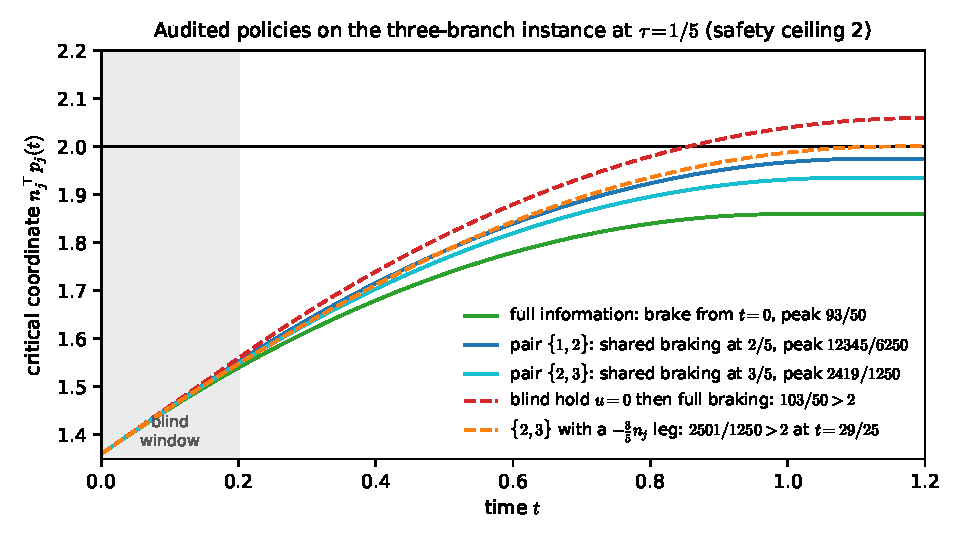
\includegraphics[width=0.92\linewidth]{fig1_trajectories.pdf}
\caption{The audited policies on the critical coordinate $\zeta_j(t)=n_j^\top p_j(t)$ at $\tau=\tfr15$, every peak the exact rational of the text: the full-information singleton peaks at $\tfr{93}{50}$; the pair policies of Proposition~\ref{prop:pairs} peak below the ceiling ($\tfr{12345}{6250}$, $\tfr{2419}{1250}$); the two falsified variants cross it ($\tfr{103}{50}$; $\tfr{2501}{1250}$ at $t=\tfr{29}{25}$). Generated by a recompute-then-assert script: every plotted peak is recomputed in rational arithmetic and asserted before the figure is written.}
\label{fig:traj}
\end{figure}

\subsection{The finite program and its exact witnesses}

Set $\tau=\tfr15$, $T=\tfr65$ and the uniform mesh $h=\tfr1{10}$: two common pre-observation blocks and ten post-observation blocks for each of three modes, so $Q=32$ and $mQ=64$; the time labels are the mesh points. For the endpoint position rows the kernel $(T-s)n_j$ is affine on every block, so the exact moment error is $e=\sum_J|J|^2/4=12\cdot h^2/4=\tfr3{100}$; the endpoint margin is $\beta=\tfr{16}{25}-\tfr65=-\tfr{14}{25}$, relaxed to $\beta+e=-\tfr{53}{100}$. The exact continuous certificate has margin $\tfr3{50}$; the finite program returns $\tfr3{100}$.

\emph{Dual witness.} Order the input facets as $F=[(0,1);(0,-1);(2,1);(2,-1);(-2,1);(-2,-1)]$, $f=(\tfr45,\tfr45,2,2,2,2)$, and set $\eta_1=(0,0,0,0,\tfr14,\tfr14)$, $\eta_2=(0,\tfr12,0,\tfr3{10},0,0)$, $\eta_3=(\tfr12,0,\tfr3{10},0,0,0)$, which satisfy $F^\top\eta_j=-n_j$ and $f^\top\eta_j=1$. For a post-observation block $J_k$ put $a_k=\int_{J_k}(T-s)\dd s$ and $\mu_{j,k}=\lambda_ja_k\eta_j$. Before observation, stationarity holds because $\sum_j\lambda_jn_j=0$; after observation, because $\lambda_ja_kn_j+F^\top\mu_{j,k}=0$. Since $\sum_ka_k=(T-\tau)^2/2=\tfr12$, the Farkas combination is $\lambda^\top(\beta+e)+\mu^\top f_{\mathrm{blk}}=-\tfr{53}{100}+\tfr12=-\tfr3{100}<0$: an exact rational certificate of infeasibility of the shifted system, i.e.\ a dual objective of $\tfr3{100}$.

\emph{Primal witness.} Hold the pre-observation blocks at $0$ and the post-observation blocks of mode $j$ at $-n_j$. The endpoint row then reads $-\tfr12+\tfr{14}{25}-\tfr3{100}=\tfr3{100}$, and every other row lies at or below that value: the velocity and noncritical position rows are continuously safe at the witness, the endpoint critical rows attain $\tfr3{100}$ with equality, and the remaining critical rows interpolate monotonically (the braking profile increases to its endpoint maximum). All $465$ rows are checked exactly by the verification script.

\subsection{The mesh law}

The witness pair is mesh-generic, and this gives a closed form for the finite value on every admissible mesh.

\begin{proposition}[mesh law on aligned meshes]\label{prop:meshlaw}
Let $\calH$ be any mesh of $[0,\tfr65]$ containing $\tau=\tfr15$, with time labels at the mesh points and exact moment errors. Then
\begin{equation}\label{eq:meshlaw}
\rho(\calH)=\tfr3{50}-\tfr14\sum_{J\in\calH}|J|^2 ,
\end{equation}
certified by the primal and dual witnesses above. In particular $\rho(h)=\tfr3{50}-Th/4$ on uniform meshes, $\rho(\calH)>0$ if and only if $\sum_J|J|^2<\tfr6{25}$, and the finite value converges to $\J=\tfr3{50}$ from below with the gap equal to the endpoint moment error.
\end{proposition}

\begin{proof}
Write $e_T=\tfr14\sum_J|J|^2$ for the endpoint moment error. The dual objective is $-(\beta+e_T)-\sum_ka_k=\tfr{14}{25}-e_T-\tfr12=\tfr3{50}-e_T$ on every aligned mesh, because $\sum_ka_k$ telescopes to $(T-\tau)^2/2$ independently of the blocks; stationarity is blockwise and does not involve the mesh. For the primal witness the endpoint critical rows attain exactly $\tfr3{50}-e_T$. A critical row at a label time $t\ge\tau$ has value $\zeta(t)-2-e_t$ with $e_T-e_t=\tfr14\sum_{J\subset[t,T]}|J|^2\le\tfr14(T-t)^2$ and $2-\zeta(t)+\tfr3{50}=\tfr12(T-t)^2$, so it lies below the endpoint value; for $t\le\tau$ the same bound gives $e_T-e_t\le\tfr9{25}<\tfr7{10}-t$. Noncritical position rows are at most $\tfr{18}{25}-2$. Velocity rows have zero moment error and value at most $1-\tfr65=-\tfr15$, which is below $\tfr3{50}-e_T$ because $e_T\le\tfr14(\tau^2+(T-\tau)^2)=\tfr{13}{50}$---with equality exactly on the two-block mesh $\{0,\tau,T\}$, where $\rho=-\tfr15$ and the velocity rows are tight. Primal value and dual objective coincide, so both are optimal.
\end{proof}

\begin{table}[t]
\centering\small
\caption{Solver-assisted, exactly certified mesh campaign on the three-branch instance ($\tau=\tfr15$, $T=\tfr65$): program dimensions ($mQ+1$ variables; $Ms(N_t{+}1)+p_UQ$ inequalities with $s=7$, $p_U=6$, $N_t=T/h$), exact optimal value from \eqref{eq:meshlaw}, value returned by the HiGHS dual simplex \cite{HuangfuHall2018} through SciPy, simplex iterations and wall-clock time (single runs on the verification machine, Linux x86\_64, Intel Xeon @ 2.60\,GHz, Python~3.13, SciPy~1.17; counts and times may vary with solver version). Optimality of each exact value is certified by the mesh-independent primal--dual witness pair, independently of the solver. At $h=\tfr15$ the witness certifies the value zero; at the finer meshes it is a positive obstruction certificate.}
\label{tab:mesh}
\begin{tabular}{@{}rrrrrrrr@{}}
\toprule
$h$ & blocks $Q$ & variables & rows & exact $\rho(h)$ & solver $\rho$ & iterations & time (s)\\
\midrule
$1/5$   & 16  & 33  & 243  & $0$                    & 0.000000000 & 36   & 0.004\\
$1/10$  & 32  & 65  & 465  & $\tfr{3}{100}=0.030$   & 0.030000000 & 78   & 0.006\\
$1/15$  & 48  & 97  & 687  & $\tfr{1}{25}=0.040$    & 0.040000000 & 119  & 0.008\\
$1/20$  & 64  & 129 & 909  & $\tfr{9}{200}=0.045$   & 0.045000000 & 141  & 0.013\\
$1/50$  & 160 & 321 & 2241 & $\tfr{27}{500}=0.054$  & 0.054000000 & 501  & 0.062\\
$1/100$ & 320 & 641 & 4461 & $\tfr{57}{1000}=0.057$ & 0.057000000 & 1062 & 0.243\\
\bottomrule
\end{tabular}
\end{table}

\begin{table}[t]
\centering\small
\caption{The mesh law off the uniform family: aligned meshes with unequal blocks, their exact values from \eqref{eq:meshlaw}, and the solver's returned values (agreement to $10^{-9}$ or better in every case). ``$1+6$'' denotes one blind block and six equal post-observation blocks. The last row is the $2^7$-fold refinement of $\{0,\tau,T\}$ that first meets the a-priori halting resolution of Remark~\ref{rem:apriori}.}
\label{tab:nonuniform}
\begin{tabular}{@{}lrrrrr@{}}
\toprule
mesh & $Q$ & variables & rows & exact $\rho(\calH)$ & solver $\rho$\\
\midrule
two blocks $\{0,\tfr15,\tfr65\}$ & 4 & 9 & 87 & $-\tfr15$ & $-0.200000000$\\
$1+5$ & 16 & 33 & 243 & $0$ & $0.000000000$\\
$1+6$ (smallest certifying program) & 19 & 39 & 282 & $\tfr1{120}$ & $0.008333333$\\
$2+7$ & 23 & 47 & 348 & $\tfr{27}{1400}$ & $0.019285714$\\
irregular $\{0,\tfr1{10},\tfr15,\tfr12,\tfr9{10},\tfr65\}$ & 11 & 23 & 192 & $-\tfr3{100}$ & $-0.030000000$\\
$2^7$-fold refinement ($h=\tfr1{128}$) & 512 & 1025 & 8469 & $\tfr{371}{6400}$ & $0.057968750$\\
\bottomrule
\end{tabular}
\end{table}

Table~\ref{tab:mesh} reports the campaign on uniform meshes and Table~\ref{tab:nonuniform} the law off the uniform family. The solver agrees with the exact values to at most $4.2\times10^{-17}$ on the campaign meshes; the agreement is a confirmation of a proved optimum, not evidence for it. Two consequences of \eqref{eq:meshlaw} are worth recording. First, because equal blocks minimise $\sum_J|J|^2$ at fixed count, the smallest aligned program with a positive certificate has one blind block and six post-observation blocks ($Q=19$, $39$ variables, $282$ rows, $\rho=\tfr1{120}$); five post-observation blocks give exactly zero. Second, time refinement on this instance has no conflict structure to target---the error is the same $|J|^2/4$ per block whatever the block---so the lever that \emph{does} have structure is the information axis, which Section~\ref{sec:ladder} reads.

\begin{figure}[t]
\centering
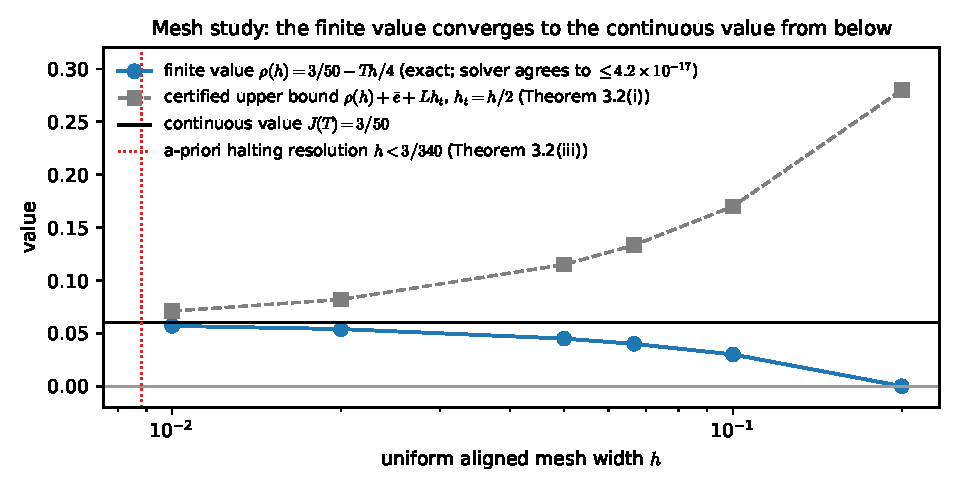
\includegraphics[width=0.88\linewidth]{fig2_meshlaw.pdf}
\caption{Mesh study on uniform aligned meshes: the finite value $\rho(h)=\tfr3{50}-Th/4$ (exact; solver agreement to $4.2\times10^{-17}$) converges to the continuous value $\tfr3{50}$ from below, while the certified upper bound $\rho(h)+\ebar+Lh_t$ of Theorem~\ref{thm:bridge}(i) (with $\ebar=Th/4$, $L=\tfr{11}5$, $h_t=h/2$) converges from above. The dotted line marks the a-priori halting resolution $h<\tfr3{340}$ of Theorem~\ref{thm:bridge}(iii); every uniform aligned mesh with $h<\tfr15$ already certifies.}
\label{fig:mesh}
\end{figure}

\subsection{Reading the sandwich on the instance}\label{sec:sandwich}

The hypothesis constants are $R_U=1$ (the hexagon's circumradius), $V_U=\tau+1=\tfr65$ (the endpoint kernels are unit-slope ramps of height $t_\ast$), $\delta_\beta=0$ (margins exact; no stored-scenario error) and $L=T+1=\tfr{11}5$: the kernel difference $k_t-k_{t'}$ has $L^1$ norm at most $T|t-t'|$ (it is \emph{not} supported on $[t',t]$; the position rows also differ by $(t-t')n_j$ on $[0,t']$), while $|\beta_t-\beta_{t'}|=|t-t'|$. With labels at the mesh points the covering radius is $h_t=h/2$. The sandwich \eqref{eq:sandwich} at $h=\tfr1{10}$ therefore bounds $J\le\tfr3{100}+\tfr3{100}+\tfr{11}{100}=\tfr{17}{100}$, while the witness pair proves that the realised gap is exactly $Th/4=\tfr3{100}$; Figure~\ref{fig:mesh} shows both sides closing.

\paragraph{Why the $\max_a\ebar_a$ form is load-bearing.}
Suppose the program had been fed the loose but verified bound $\ebar=e+\tfr12$ on every row. It then returns $\rho=-\tfr{47}{100}$ at $h=\tfr1{10}$, and the certified bound $J\le\rho+\ebar+\delta_\beta+Lh_t=\tfr{17}{100}\ge\tfr3{50}$ remains valid, whereas the uniform special case $R_UV_Uh_u$ would claim $J\le-\tfr6{25}$---false at $J=\tfr3{50}$. A loose relaxation must inflate the charged bound with it.

\begin{remark}[a-priori versus realised resolution]\label{rem:apriori}
Theorem~\ref{thm:bridge}(iii) guarantees a certificate of margin at least $\gamma/2=\tfr3{100}$ once $(R_UV_U+L)h<\gamma/2$, i.e.\ $h<\tfr3{340}\approx0.0088$; on the dyadic refinements of $\{0,\tau,T\}$ this is first met at $h=\tfr1{128}$ (Table~\ref{tab:nonuniform}, $\rho=\tfr{371}{6400}$). The realised law \eqref{eq:meshlaw} attains the same margin already at $h=\tfr1{10}$ and certifies on every uniform aligned mesh with $h<\tfr15$. The a-priori bound is thus conservative here by a factor of about $11$ in mesh width ($\tfr1{10}$ against $\tfr3{340}$)---expected, since it charges the time-interpolation term $Lh_t$ that the witness pair shows to be inactive on this instance. The a-priori bound is what makes nonviability \emph{semidecidable} in the class; the realised law is what makes it \emph{cheap}.
\end{remark}

\subsection{Support of the certificates on the instance}

\begin{corollary}[minimal support]\label{cor:support}
At $\tau=\tfr15$ every positive certificate of the triple involves all three modes, and three labels suffice: the minimal support is exactly $3=\depth_\calI(B_0)$, while the finite safety-row matrix at $h=\tfr1{10}$ has full column rank $r=64$, so Theorem~\ref{thm:bridge}(v) allows $65$.
\end{corollary}

\begin{proof}
Proposition~\ref{prop:depth} with Proposition~\ref{prop:pairs} (every pair viable) gives the lower bound; the certificate of Proposition~\ref{prop:triple} gives the upper bound; the rank is computed exactly by Gaussian elimination in the verification script.
\end{proof}

The three-label support of each positive finite certificate in Table~\ref{tab:mesh} is therefore not an accident of the symmetric campaign but the depth of the belief, and the gap between $3$ and $65$ illustrates the remark after Proposition~\ref{prop:depth}: the rank bound is a worst case over all row systems of the given dimensions, the depth is the instance's own conflict structure.
\section{Reading the certificate prescriptively}\label{sec:ladder}

A positive certificate is more than a verdict. Its weights, kernels and facet multipliers encode what a controller would have to change---where the shared authority is spent, which sub-beliefs tolerate which delays, and which observers would dissolve the obstruction. On the instance the decoding is exact end to end.

\subsection{The shared-authority ladder}

\begin{proposition}[shared-authority ladder]\label{prop:ladder}
\begin{enumerate}[label=\textup{(\roman*)},leftmargin=2.2em,itemsep=1pt]
\item The pooling weights satisfy $\sum_j\lambda_jn_j=0$ with $\lambda_j>0$; hence for every common control $w\in U$ some branch has $n_j^\top w\ge0$. No common control brakes all three branches, and the certificate's zero charge on the blind window is exactly this unbrakeability.
\item The optimal shared braking authorities $t^\ast(B)=\max_{w\in U}\min_{j\in B}(-n_j^\top w)$ are $t^\ast(\{1,2\})=t^\ast(\{1,3\})=\tfr25$, attained at $w=(-\tfr25,\mp\tfr45)$, and $t^\ast(\{2,3\})=\tfr35$, attained at $w=n_1$; $t^\ast(\{1,2,3\})=0$. The blind-window controls of Proposition~\ref{prop:pairs} are exactly these optima.
\item Braking at authority $t^\ast$ through a blind window of length $\tau$ and at $-n_j$ afterwards holds the critical peak at
\[
\zeta^{\max}(\tau)=\tfr{93}{50}+(1-t^\ast)\tau+\tfr{(t^\ast)^2-t^\ast}{2}\tau^2 ,
\]
increasing in $\tau$ on $[0,1/t^\ast]$; it reaches the ceiling $2$ at $\tau_{12}=\tau_{13}=\tfr{15-\sqrt{183}}{6}\approx0.2454$ and $\tau_{23}=\tfr{10-\sqrt{58}}{6}\approx0.3974$, against the triple's $\tau^\ast=\tfr7{50}$; singletons are delay-independent.
\end{enumerate}
\end{proposition}

\begin{theorem}[exact two-branch thresholds at the fixed horizon]\label{thm:pairs}
For the plant and observation protocol of Section~\ref{sec:instance} at $T=\tfr65$, the beliefs $\{1,2\}$, $\{1,3\}$ and $\{2,3\}$ admit a safe measurable observation-adapted controller precisely when $\tau\le\tfr{15-\sqrt{183}}6$, $\tau\le\tfr{15-\sqrt{183}}6$ and $\tau\le\tfr{10-\sqrt{58}}6$ respectively. No assumption of blockwise-constant control is needed for the impossibility direction.
\end{theorem}

Both results are proved in Appendix~\ref{app:ladder}. The impossibility half of Theorem~\ref{thm:pairs} is a two-label dual: with $t=t^\ast(B)$, normalised weights on the two critical facets ($(\tfr38,\tfr58)$ for pairs containing branch~1, $(\tfr12,\tfr12)$ for $\{2,3\}$) and a common label time $s_\ast=1+(1-t)\tau$,
\begin{equation}\label{eq:pairdual}
\Gamma_B(\tau)=-t\int_0^\tau(s_\ast-s)\dd s-\int_\tau^{s_\ast}(s_\ast-s)\dd s-\Bigl(\tfr{16}{25}-s_\ast\Bigr)=-\tfr7{50}+(1-t)\tau-\tfr{t(1-t)}2\tau^2 ,
\end{equation}
which minimises over \emph{every} measurable common blind control and every independently chosen post-revelation control, and whose first zero is the displayed root; delays beyond the root are handled by Lemma~\ref{lem:mono}. The viability half is the explicit schedule of (iii), verified facet by facet on the closed interval up to the root. The identity $\Gamma_B(\tau)=\zeta^{\max}(\tau)-2$ shows that dual and schedule are tight against each other at every delay, not only at the threshold.

\begin{figure}[t]
\centering
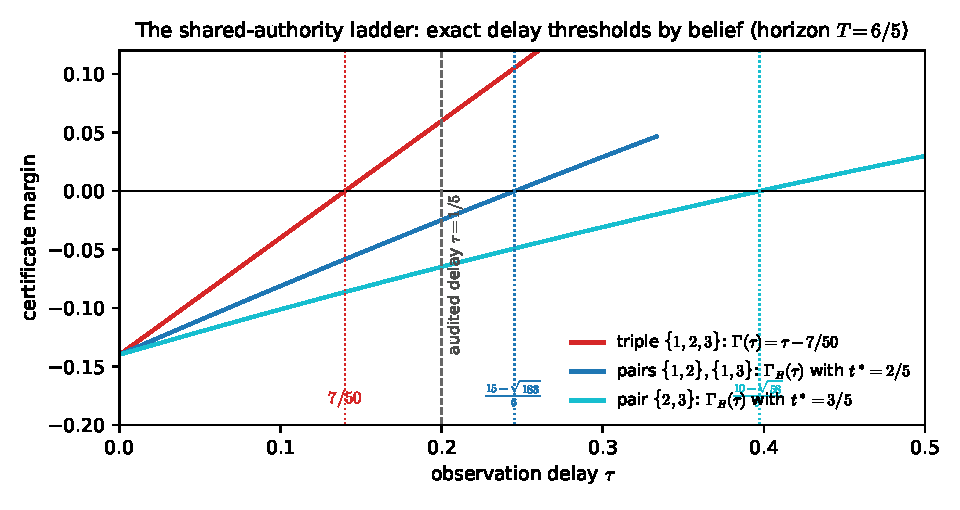
\includegraphics[width=0.88\linewidth]{fig3_ladder.pdf}
\caption{The shared-authority ladder. Certificate margins as functions of the observation delay: the triple's $\Gamma(\tau)=\tau-\tfr7{50}$ and the two-label pair duals $\Gamma_B(\tau)$ of \eqref{eq:pairdual}, plotted where their label time stays inside the horizon. Zero crossings are the exact thresholds $\tfr7{50}<\tfr{15-\sqrt{183}}6<\tfr{10-\sqrt{58}}6$; the audited delay $\tau=\tfr15$ lies strictly inside both pair rungs and outside the triple's.}
\label{fig:ladder}
\end{figure}

\paragraph{The prescriptive reading.}
The obstruction is removed by any of three levers, and the certificate prices each. \emph{Shorten the window} below the relevant rung: the pairs already tolerate $\tau=\tfr15$ under shared braking alone. \emph{Add observers}: each information refinement deletes rungs, and the erosion identity below says exactly which splits pay. \emph{Reallocate authority where the certificate charges it}: the post-window controls already brake at the hexagon's face $-n_j\in U$, the dual's $\eta_j$ place their mass on the braking facets $\mp n_j$, and the primal witness brakes every mode to rest, so the binding resource is the shared window, not the post-observation actuator.

\subsection{Pricing observers: the erosion identity}\label{sec:erosion}

Suppose an information cell $C$ is split into finer cells $C_1,\dots,C_k$ on an interval $I\subseteq[0,T]$---an observer installed on $I$. Because $\phi_U$ is superadditive, $\phi_U(g_1+\dots+g_k)\ge\sum_j\phi_U(g_j)$, the \emph{same} witness has a smaller margin on the finer structure, and the loss is exact:
\begin{equation}\label{eq:erosion}
\Gamma_{\mathrm{coarse}}-\Gamma_{\mathrm{fine}}=\int_I\Bigl[\phi_U\Bigl(\sum_jg_{C_j}(t)\Bigr)-\sum_j\phi_U\bigl(g_{C_j}(t)\bigr)\Bigr]\dd t\;\ge0 .
\end{equation}
For $U=[-\bar u,\bar u]^m$ the integrand is $\bar u\bigl[\sum_j\|g_{C_j}(t)\|_1-\|\sum_jg_{C_j}(t)\|_1\bigr]$: the certificate identifies the time intervals on which indistinguishable branches demand conflicting control effort. Equation~\eqref{eq:erosion} is a statement about one witness, not about the optimised value: a coarse cell can strengthen an obstruction, and splitting it can dissolve the certificate while the system's verdict is unchanged (an optimised certificate may exist for the finer structure). Its discrete counterpart is the master monotonicity of \cite{Abaee2026worked}. On the instance the identity is computable in closed form, because every pooled kernel is $(t_\ast-s)$ times a fixed vector.

\begin{proposition}[erosion of the triple certificate under time-zero observers]\label{prop:erosionrows}
Let the blind cell $\{1,2,3\}$ of the instance ($\tau=\tfr15$) be replaced from time $0$ by a finer partition. The erosion \eqref{eq:erosion} of the certificate of Proposition~\ref{prop:triple} and the resulting margin are:
\begin{center}\small
\begin{tabular}{@{}lccc@{}}
\toprule
observer (partition of the blind cell) & integrand constant & erosion & eroded margin\\
\midrule
$\{1\}\,|\,\{2,3\}$ & $\tfr34$ & $\tfr{33}{200}=0.165$ & $-\tfr{21}{200}$\\
$\{2\}\,|\,\{1,3\}$ and $\{3\}\,|\,\{1,2\}$ & $\tfr58$ & $\tfr{11}{80}=0.1375$ & $-\tfr{31}{400}$\\
$\{1\}\,|\,\{2\}\,|\,\{3\}$ (full revelation) & $1$ & $\tfr{11}{50}=0.22$ & $-\tfr4{25}$\\
\bottomrule
\end{tabular}
\end{center}
Every time-zero observer dissolves the certificate, consistently with Proposition~\ref{prop:pairs} (each remaining cell is a viable sub-belief), and the observer ranking by erosion---$\{1\}|\{2,3\}$ first---agrees with the ladder ranking by delay tolerance, $\tau_{23}>\tau_{12}$.
\end{proposition}

\begin{proof}
With $k_j=(t_\ast-s)n_j$ and $\lambda=(\tfr38,\tfr5{16},\tfr5{16})$ the coarse pooled kernel vanishes, so $\phi_U=0$ on the blind window. For the cells of a split, $\phi_U\bigl((t_\ast-s)\sum_{j\in C}\lambda_jn_j\bigr)=-(t_\ast-s)\,h_U\bigl(-\sum_{j\in C}\lambda_jn_j\bigr)$: the singleton $\{1\}$ gives $\tfr38$; the pair $\{2,3\}$ pools to $(-\tfr38,0)$, whose support value is $\tfr38$; the pair $\{1,3\}$ pools to $(\tfr3{16},-\tfr14)$, whose support value is $\tfr5{16}$, as does the singleton $\{2\}$; full revelation gives $\sum_j\lambda_j=1$. Multiplying by $\int_0^\tau(t_\ast-s)\dd s=\tau+\tau^2/2=\tfr{11}{50}$ gives the table.
\end{proof}

The identity also prices an observer installed \emph{later} than time zero, because the split is then active only on $[\tau_1,\tau]$ and the integral in \eqref{eq:erosion} is taken over that interval. This turns the certificate into a design tool with a certified answer.

\begin{proposition}[an observer installed at $\tau_1$]\label{prop:observer}
Let the instance ($\tau=\tfr15$, $T=\tfr65$) be modified so that at time $\tau_1\in[0,\tau]$ the controller learns whether the mode is $1$ (partition $\{1\}|\{2,3\}$), full revelation remaining at $\tau$. Then:
\begin{enumerate}[label=\textup{(\alph*)},leftmargin=2.2em,itemsep=1pt]
\item the triple certificate eroded on $[\tau_1,\tau]$ has margin
\[
\Gamma(\tau_1)=\tfr3{50}-\tfr34\int_{\tau_1}^{\tau}(t_\ast-s)\dd s=\tfr3{50}-\tfr38\Bigl[\bigl(\tfr65-\tau_1\bigr)^2-1\Bigr],
\]
increasing in $\tau_1$, with $\Gamma(0)=-\tfr{21}{200}$, $\Gamma(\tfr15)=\tfr3{50}$ and a unique zero at $\tau_1^{\mathrm{dual}}=\tfr{6-\sqrt{29}}5\approx0.12297$; the triple is certified nonviable for every $\tau_1>\tau_1^{\mathrm{dual}}$;
\item the schedule ``common control $w=(\tfr3{20},0)$ on $[0,\tfr3{25}]$; then $u=-n_1$ to rest in cell $\{1\}$, $u=n_1$ on $[\tfr3{25},\tfr15]$ in cell $\{2,3\}$ followed by $u=-n_j$ to rest'' is safe for $\tau_1=\tfr3{25}$: branch~1 peaks at $\tfr{999621}{500000}=1.999242$, branches~2 and~3 at $\tfr{24993709}{12500000}\approx1.999497$, all seven facets holding on all three branches; by Lemma~\ref{lem:mono} the triple is viable for every $\tau_1\le\tfr3{25}$;
\item hence the critical installation time $\tau_1^\ast$ satisfies $\tfr3{25}\le\tau_1^\ast\le\tfr{6-\sqrt{29}}5$, an interval of width less than $3\times10^{-3}$.
\end{enumerate}
\end{proposition}

\begin{proof}
(a) On $[0,\tau_1]$ the pooled kernel vanishes; on $[\tau_1,\tau]$ the cells $\{1\}$ and $\{2,3\}$ contribute $-\tfr38(t_\ast-s)$ each (the constants of Proposition~\ref{prop:erosionrows}); after $\tau$ the certificate is unchanged. The integral is $\tfr12[(t_\ast-\tau_1)^2-(t_\ast-\tau)^2]$ with $t_\ast=\tfr65$, which gives the displayed form; positivity is the certificate statement of Lemma~\ref{lem:semantics} for the two-stage information structure, which is admissible in Theorem~\ref{thm:bridge} (partitions refine in time). (b) is an exact computation (SM~S4): the window exit velocities are $\tfr{509}{500}$ for branch~1 and $\tfr{2473}{2500}$ for branches~2,~3, the shared braking leg lowers the latter to $\tfr{2353}{2500}$, and braking to rest adds half the squares. An observer installed earlier than $\tfr3{25}$ may be ignored until $\tfr3{25}$. (c) combines (a) and (b).
\end{proof}

\begin{figure}[t]
\centering
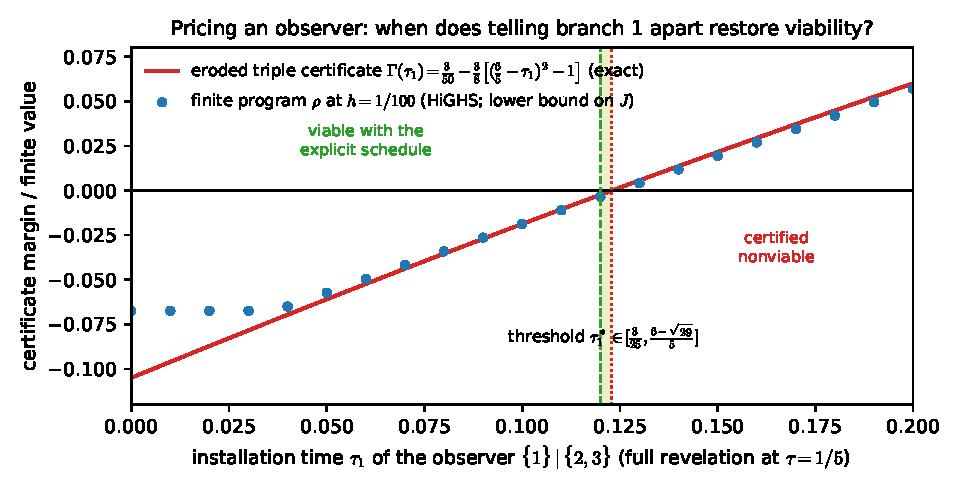
\includegraphics[width=0.88\linewidth]{fig4_observer.pdf}
\caption{Pricing an observer. The eroded certificate $\Gamma(\tau_1)$ of Proposition~\ref{prop:observer}(a) (exact), and the finite program of \eqref{eq:lp} built for the two-stage information structure at $h=\tfr1{100}$ (HiGHS; each point a lower bound on $J$). For $\tau_1\le\tfr3{100}$ the program finds a better certificate than the eroded triple one---its value settles at the finite value of the pair $\{2,3\}$'s own program, $-0.0675$, within the moment error of that pair's slack $-\tfr{81}{1250}$---while for $\tau_1\ge\tfr1{10}$ the two agree up to the moment error $Th/4=\tfr3{1000}$. The shaded band is the certified bracket $[\tfr3{25},\tfr{6-\sqrt{29}}5]$ for the critical installation time.}
\label{fig:observer}
\end{figure}

Figure~\ref{fig:observer} adds the finite program's own answer: built for the two-stage structure at $h=\tfr1{100}$, it returns $\rho>0$---a solver-found, exactly checkable certificate---for every $\tau_1\ge\tfr{13}{100}$, and it dominates the eroded triple certificate everywhere ($\rho\ge\Gamma(\tau_1)-Th/4$, the latter being a dual-feasible point of the program). The program is more than the fixed-weight dual: for early installation it discovers that the binding sub-belief has become the pair $\{2,3\}$ and reports that pair's margin instead. What neither can do by itself is certify \emph{viability} below the threshold; that is the role of the explicit schedule in (b), and the width of the resulting bracket measures how tight the two-label dual is on this instance.

\subsection{What the certificate does not say}\label{sec:scope-dilation}

Two cautions keep the prescriptive reading honest. First, \eqref{eq:erosion} prices the \emph{control-kernel} grouping only; when an observer also changes the row labels (as a belief-cell enclosure does, Section~\ref{sec:extensions}), the label term moves separately. Second, the certificate's algebraic form must not be extrapolated beyond the instance that was certified. On the audited instance the dual's pre-window kernel vanishes because $\sum_j\lambda_jn_j=0$, so its pre-window expression is insensitive to an enlargement of the shared control set, and its velocity-row multipliers are zero; these are properties of that certificate, not a sensitivity law for redesigns. The expression $\Gamma_a(\tau)=\tau-\tfr7{50}-\tfr{a-1}2$ obtained by formally dilating the input set to $aU$ has zeros at $\tfr7{50},\tfr{39}{100},\tfr{16}{25}$ for $a=1,\tfr32,2$, but these are not viability thresholds at the fixed horizon: at $a=2$, $\tau=\tfr{16}{25}$ the weighted critical position reaches $2$ at $t=\tfr{16}{25}$ and exceeds $\tfr{209}{100}$ by $t=\tfr{37}{50}<T$ even if every branch is granted an independent control in $2U$ (SM~S6). Redesign claims require a new certificate or a new schedule, which is exactly what Proposition~\ref{prop:observer} supplies for the observer lever.
\section{Sound extensions beyond exogenous mode observation}\label{sec:extensions}

The exact theorem assumes that information about the mode arrives exogenously, through history partitions that do not depend on the trajectory. Two extensions keep soundness---a positive margin still proves nonviability---while giving up completeness.

\subsection{Oracle recourse after a blackout}

Suppose finitely many admissible initial-state/disturbance scenarios are provably indistinguishable until $\tau$ in the sense that they generate identical observation histories, with arbitrary (possibly state-dependent) sensing afterwards. Grant the controller, after $\tau$, a separate arbitrary control signal for every stored scenario: an \emph{oracle relaxation} of the true policy class, which reveals the realised scenario at $\tau$ even where scenarios remain observationally identical. Every real output-feedback policy induces one common pre-$\tau$ control and is therefore contained in the oracle class, so nonviability in the enlarged class transfers down. Concretely, if
\begin{equation}\label{eq:oracle}
\int_0^\tau\phi_U\Bigl(\sum_\ell\lambda_\ell k_\ell\Bigr)\dd t+\sum_\ell\int_\tau^T\phi_U(\lambda_\ell k_\ell)\dd t-\sum_\ell\lambda_\ell\beta_\ell>0 ,
\end{equation}
with $\beta_\ell$ computed from the explicitly stored scenario $\ell$, then no actual output-feedback policy is safe (SM~S5). The certificate covers arbitrary sensing after a known blackout; it is sound but in general incomplete, because the oracle class is strictly larger than the true one. On the instance the exactness of the threshold belongs to the complete revelation at $\tau$, not to the relaxation.

\subsection{Belief cells}

A third extension replaces the exact scenario store---and the exact revelation of the audited model---by a certified \emph{belief cell}: a set $C\subseteq\Theta\times\R^n$, carried with a polytope enclosure, that the observation history certifies to contain the true mode--state pair. This is a set-valued observer with a guaranteed error radius in the sense of the bounding approaches to estimation \cite{Witsenhausen1968,Milanese1996}.

\begin{proposition}[conditional belief-cell certificates]\label{prop:beliefcells}
Let each cell label be an explicitly verified outer row enclosure for its compatible mode--state pairs. With \textup{(H6)} checked for these labels---including a separate bound on the full label discrepancy---the corresponding finite program is linear (conic for certified cell support functions), and the lower bound and positive-margin obstruction of Theorem~\ref{thm:bridge} apply to the cell-filtration policy class. An upper sandwich requires the same separately verified \textup{(H6)} budget and an implementable held-policy comparison; it does not follow from a cell radius alone. Splitting cells changes both the row labels and the control-kernel grouping, so \eqref{eq:erosion} accounts for the latter term only. A safety-margin claim for a primal witness requires its actual held-policy row slack and an enclosure error no larger than that slack; a dual margin survives only after all enclosure errors charged by its normalised weights remain smaller than the margin.
\end{proposition}

The proof (SM~S5) is the one-sided relaxation argument of Theorem~\ref{thm:bridge}(ii) applied row by row, together with an example showing that the label term can move by $\tfr34$ under a split whose kernel term is zero. On the instance the belief cells are the compatible-mode sets, and the instance provides a complete cell-refinement family: the full cell $\{1,2,3\}$ obstructs past $\tfr7{50}$, the two-mode cells have the exact all-control thresholds of Theorem~\ref{thm:pairs}, and the singletons never obstruct. For a proposed \emph{noisy} state cell the slacks $\tfr{31}{1250}$ and $\tfr{81}{1250}$ of the pair policies and the dual margin $\tfr3{50}$ of the triple may be used as budgets only after the cell's held-policy slack and full row-label errors have been enclosed separately; a nominal position radius is not by itself a proof of the needed error bound.

\subsection{Scope}\label{sec:scope}

The exact theorem does not cover control-dependent observations or active sensing; arbitrary continuous-state measurements; nonlinear dynamics without additional validated enclosures (a uniform validated flow-error bound added to the row budgets yields a sound extension, not automatic completeness); nonconvex actuator sets without a relaxation gap (convexity is structural: block averages of admissible controls lie in $\conv U$, and the weak-$\ast$ compactness of Proposition~\ref{prop:value} uses that $U$ is a compact convex polytope); rate-constrained actuators without modifying the approximation; or unrestricted infinite-horizon completeness. Against the alternatives: full-information viability is necessary but not sufficient; initial-admissibility and tangency tests are silent on the instance's obstruction, which is temporal--informational rather than pointwise-geometric; safety-before-first-observation tests are silent when a common safe blind control exists; exact finite safety games under imperfect information \cite{Chatterjee2007} exist as discrete models, and what is needed to use them as sound abstractions of the present continuous systems is precisely a justified continuous-to-finite bridge; and naive held-control infeasibility excludes only the held-control class. No general-purpose computational-calculus claim is made: Theorem~\ref{thm:bridge} is a certificate generator for the stated class, complete under refinement and semidecidable with effectively computable bounds.
\section{Computation and verification}\label{sec:computation}

\subsection{Complexity and the residual-bounded certificate test}

With $Q$ information--time blocks and $N_t+1$ time labels, program \eqref{eq:lp} has $mQ+1$ variables and at most $Ms(N_t{+}1)+p_UQ$ inequalities; it is solvable in time polynomial in these dimensions and in the encoded rational data size (weakly polynomial bit complexity) for exact rational data, and for interval-enclosed inputs once the enclosures are fixed. Initial-state dependence is affine, so no vertex enumeration of $P_\theta$ is required: at each label one solves $\max_{\xi\in P_\theta}c_i^\top X_\theta(t,0)\xi$ and stores a maximising or near-maximising point---the verifier needs only membership of the stored point in $P_\theta$, not its optimality; near-optimality bears on completeness, not on the validity of a positive certificate. The same holds for stored disturbance signals.

For rational outer rows $\widehat Av\le\widehat b$, $F_{\mathrm{blk}}v\le f_{\mathrm{blk}}$, a \emph{residual-bounded} test suffices to validate a certificate without exact stationarity: with $\lambda,\mu\ge0$, $r=\widehat A^\top\lambda+F_{\mathrm{blk}}^\top\mu$ and $c=\lambda^\top\widehat b+\mu^\top f_{\mathrm{blk}}$,
\begin{equation}\label{eq:residual}
c+\sum_jh_U(-r_j)<0
\end{equation}
is sufficient, since every feasible $v$ satisfies $-\sum_jh_U(-r_j)\le r^\top v\le c$. The actuator rows already encode $v_j\in U$; their multipliers in \eqref{eq:residual} are redundant but legitimate, and the verifier uses both paths as independent cross-checks. All integration, rounding and model-enclosure errors must be included before the test is applied, and uncertain row data must be relaxed \emph{toward a larger feasible controller set}: overestimating the worst disturbance contribution can create a false obstruction, which is the sign convention behind $\beta^+_a\ge\beta_a$. A deletion-based sparsification attempts supported labels for deletion one at a time in a fixed order, keeping a deletion only if the prescribed target margin survives the feasibility re-solve; it terminates with an irredundant (not claimed minimal) support at one feasibility solve per safety row. If $\J=\gamma>0$, any mesh with $\max_a\ebar_a+R_DV_Dh_d+\delta_{\mathrm{init}}+\delta_{\mathrm{num}}+Lh_t<\gamma$ guarantees detection: an explicit margin-dependent resolution bound, not a certificate-size bound.

\subsection{Verification architecture}\label{sec:verification}

The division of labour is fixed by design.

\paragraph{Exact witnesses, not solver output.}
Every reported mathematical value---thresholds, peaks, slacks, program dimensions, the mesh law, the erosion table, the observer bracket---is re-derived by the verification script \texttt{paper03\_computational\_certification\_v23\_verification.py} in exact rational arithmetic (Python \texttt{fractions}; 63 checks, all passing), which also rebuilds program \eqref{eq:lp} at every mesh of Tables~\ref{tab:mesh}--\ref{tab:nonuniform} and for the two-stage information structure of Proposition~\ref{prop:observer}, evaluates the primal and dual witnesses row by row, computes the rank of the safety-row matrix by exact Gaussian elimination, and---optionally, if SciPy is present---runs the HiGHS dual simplex \cite{HuangfuHall2018} and compares its returned optimum with the exact value. The solver's agreement ($4.2\times10^{-17}$ on the campaign) is a confirmation; the proof is the witness pair. This is the same stance as exact rational LP verification \cite{Applegate2007}, with the difference that here the witnesses are closed-form and mesh-generic, so no exact simplex is needed. The figures are produced by a recompute-then-assert script that re-derives every plotted peak, threshold and crossing before drawing (SM~S7).

\paragraph{A mechanised core.}
The Farkas soundness direction on which the exact witnesses rest---a nonnegative combination of the rows with negative right-hand side excludes every feasible point---is proved in a Lean~4 \cite{deMouraUllrich2021} layer from the ordered-field interface alone (60 modules; a comment-aware scan finds no \texttt{sorry}, \texttt{admit} or ad hoc axiom; three \texttt{native\_decide} uses in support examples extend kernel-only trust to the compiler and are declared as such). The converse direction, the value identity, the bridge theorem and the belief-cell proposition call for analysis (weak-$\ast$ compactness, exponentials) that the interface does not supply and are cited rather than formalised; SM~S7 records the pinned build and its gates.

\paragraph{The finite-side reference library.}
The finite machinery that the bridge reduces to---the exact backward recursion of the calculus and the fibre-partition monitoring criteria---is packaged as \texttt{viacert}, a standard-library-only Python package using exact integer and rational arithmetic, with a pluggable \texttt{FiniteSystem} interface and a self-test of twelve audited identities inherited from the companion audits \cite{Abaee2026calc,Abaee2026worked}. In the certification workflow it plays the enumerate-and-check role; it is deliberately \emph{not} a reimplementation of the continuous programs, which live in the campaign scripts. Three tooling directions are recorded rather than implemented: warm-started incremental refinement (re-solve on block splits seeded with the coarse dual), an arbitrary-precision dual re-solve for interval-coefficient programs, and conflict-targeted block refinement where kernels are non-affine.
\section{Related work}\label{sec:related}

The construction has four properties---finite, solver-attainable, independently checkable, valid against every measurable information-adapted policy---and each of the first three has an established literature. This section places the construction relative to each and states what is and is not claimed.

\paragraph{Viability kernels and two-sided approximation.}
Saint-Pierre's viability kernel algorithm \cite{SaintPierre1994} approximates the finite-horizon kernel by a backward recursion on a grid with a convergence statement for open constraint sets; level-set formulations compute the same objects through Hamilton--Jacobi equations \cite{MitchellBayenTomlin2005}; Lagrangian reformulations in terms of reachable sets scale considerably further \cite{Maidens2013}; and the convex theory of set invariance is surveyed in \cite{Blanchini1999}. \textbf{The two-sided structure is not new, and this paper does not claim it is.} Reachability-based computations produce a guaranteed under-approximation of the kernel together with an over-approximation and use the latter to bound the error of the former \cite[Section~3]{Maidens2013}; the sandwich \eqref{eq:sandwich} is of that kind. What differs is the object and the approximations. Classical schemes discretise a \emph{state space} and approximate a \emph{kernel}; here the discretisation is an outer moment relaxation of information-adapted \emph{controls} together with an inner adversarial selection of labels and scenarios, and the quantity bounded is a safety \emph{value} over an information state. The partial-observation structure, and the requirement that the certificate hold against every measurable policy rather than against one synthesised controller, is what forces the change. Occupation-measure formulations turn optimal control into infinite-dimensional linear programs \cite{Vinter1993} whose LMI relaxations converge \cite{Lasserre2008}, and outer approximations of maximum controlled-invariant sets have been computed this way for polynomial systems \cite{Korda2014}; those are full-information constructions, and their relaxations are semidefinite rather than linear.

\paragraph{Moment relaxations.}
Relaxing a hard problem into convex problems whose values converge monotonically is the moment--SOS programme \cite{Lasserre2001,Parrilo2003}, whose hierarchy produces nondecreasing lower bounds with asymptotic convergence and, importantly, checkable rank and flat-extension conditions under which a relaxation is certified exact. That certification idea is the direct ancestor of the present one, and the differences are concrete: the hierarchy applies to polynomial optimisation over semi-algebraic sets and is solved by semidefinite programming, whereas the relaxations here are \emph{linear} programs over block moments of a linear system; convergence there is in relaxation degree, here along a refinement sequence whose mesh and stored-scenario widths vanish; and an exactness certificate there licenses the extraction of a minimiser, whereas a positive margin here is an \emph{obstruction} certificate.

\paragraph{The scenario approach, and why the guarantee here is not probabilistic.}
Sampling finitely many uncertainty instances and solving the resulting finite program is the scenario approach \cite{CalafioreCampi2005,CalafioreCampi2006}, with sharp sample-complexity results \cite{CampiGaratti2008,CampiGaratti2011,CampiGarattiPrandini2009}. The inner approximation here---finitely many stored labels and scenarios---is superficially the same move but not the same guarantee. The scenario guarantee is probabilistic: violation of the unsampled constraints with probability at most $\epsilon$, with confidence $1-\beta$. The guarantee here is worst-case: scenarios are selected adversarially rather than sampled, the bound holds for every measurable policy, and $\ebar$, $\delta_\beta$ and $Lh_t$ are deterministic inflation certificates, not violation probabilities. (The notational collision on $\beta$ is flagged rather than resolved.)

\paragraph{Minimax reachability, set-membership estimation, and imperfect-information games.}
The quantifier order $\exists$ control $\forall$ disturbance with set-membership uncertainty goes back to \cite{BertsekasRhodes1971}; set-valued state estimation under perturbed observations to \cite{Witsenhausen1968} and the bounding approaches in \cite{Milanese1996}, which are the natural source of the belief cells of Section~\ref{sec:extensions}. In robust linear optimisation, the gap between static and adjustable decisions has a theorem-of-the-alternatives characterisation \cite{WeiZhang2024}; the certificates here measure an information gap of the same nature---a common control forced across indistinguishable branches---but for continuous-time information structures and against measurable policies. Exact algorithms for safety games with imperfect information on finite graphs are available \cite{Chatterjee2007}; what the present paper supplies is the bridge that would make such a finite game a sound abstraction of a continuous system with a measurable policy class. The sufficiency side under imperfect measurement is \cite{Veliov1993}; the necessity side in continuous time is \cite{Abaee2026calc}, whose certificates this paper computes, and whose discrete audits \cite{Abaee2026worked} and measure-dual companion \cite{Abaee2026minimax} are cited where their results are used.

\paragraph{Verified numerics and exact linear programming.}
Enclosing the solution of a continuous problem in rigorously bounded intervals is the programme of interval arithmetic and validated integration; this paper deliberately does not use it. Every exact verification path runs in integer and rational arithmetic and optimality is certified by independent primal and dual witnesses, in the spirit of exact rational LP solution \cite{Applegate2007} but without an exact simplex, because the witnesses are closed-form. The solver is not a proof object. This is a statement about the division of labour, not a claim that interval methods are inferior; they address problems this pipeline does not, and SM~S2 shows where validated enclosures would enter the row budgets.

\paragraph{What is claimed.}
(1) A continuous-to-finite bridge for information states with a two-sided certified bound and convergence along any admissible refinement sequence (Theorem~\ref{thm:bridge}). (2) Dual feasibility as a universal certificate, and an exact atomic dual representation of the value (Corollary~\ref{cor:dual}). (3) Certificate size governed by information--time rank, with a saturating scalar-input construction and a matching depth lower bound (Section~\ref{sec:size}); the negative half---that a single input does not bound the witness count---is the part most likely to surprise. (4) A prescriptive decoding: shared authorities, an exact delay hierarchy, and observer pricing with a certified bracket (Section~\ref{sec:ladder}). (5) Exact verification paths by construction, with the solver demoted to confirmation. Not claimed: the sandwich idea as such, moment relaxation as such, scenario discretisation as such, or interval enclosure.
\section{Discussion and conclusion}\label{sec:discussion}

\paragraph{The transferable claim.}
The cost of certifying nonviability under incomplete observation is not governed by the size of the system, and it is worth saying precisely what it \emph{is} governed by, because the two are routinely conflated. The minimal support of a certificate is squeezed between the obstruction depth of the belief and the information--time rank of the declared relaxation (Proposition~\ref{prop:depth}); the number of scalar inputs bounds neither (Proposition~\ref{prop:rank}). This is a statement about certificate support, not a dimension-independent bound on assembling or solving the program: state, disturbance and discretisation still set the computational cost. The same conclusion is reached independently, in a different language and for a different certificate form, in the measure-dual companion \cite{Abaee2026minimax}, where the witness size is set by the control dimension with a tight $k+1$ bound. Two constructions, one moral: \emph{obstruction certificates are small objects whose size is fixed by the decision and information structure, not by the size of the world.}

\paragraph{What the claim rests on.}
A sound and independently checkable certification pipeline under incomplete observation rests on three requirements, and the bridge theorem delivers all three. The finite controller class must be an \emph{outer} relaxation while the stored adversarial tests are genuinely admissible scenarios---relax the controller, not the adversary, or the certificate certifies nothing. Optimality must be certifiable independently of the solver, by exact witnesses that close the gap. And certificate size must be understood in the information--time product.

\paragraph{What the instance adds.}
The three-branch instance is small enough to be carried exactly and rich enough that every weaker test passes: full-information viability holds, a common blind control is safe, every pair is viable, and held-control infeasibility is the wrong direction. The certificates detect the obstruction anyway, the mesh law explains the whole refinement gap in one line, the solver returns the proved optima to machine precision, and the prescriptive reading---the ladder, the erosion table, the observer bracket---turns a verdict into design numbers. The observer result in particular shows the certificate doing something a kernel computation does not: it prices a sensing decision with a two-sided, exactly verified answer.

\paragraph{What remains open.}
Completeness beyond refinement: an inner approximation of the policy class that is computationally effective for general (state-dependent) sensing is not known, and the oracle-recourse relaxation is the current sound surrogate. Three extension directions are recorded, each a construction of its own rather than an increment of the framework. \emph{Stochastic disturbances}: replacing support-function rows by second-moment bounds turns the program into a conic one, with exact rational witnesses replaced by conic dual certificates; the exact optima of the present campaign remain the benchmark such relaxations must meet. \emph{Decentralised controller sets, infinite-horizon and periodic regimes, nonconvex or piecewise-smooth actuators}: each alters a structural input of the bridge theorem---weak-$\ast$ compactness of the policy space, finite-horizon completeness, or convexity of the actuator set. \emph{A cross-tool benchmark}: the instance, with its certificate file as the exchange format, is a natural common test for exact finite safety games, interval-reachability toolchains and SMT-backed barrier synthesis; the independent certificate-file parser and the tooling directions of Section~\ref{sec:verification} are its computational prerequisites.

\paragraph{Conclusion.}
Under incomplete observation, nonviability can be certified by a finite linear program whose dual solutions cover every measurable information-adapted policy, whose refinement is complete, whose optimality is checkable in exact arithmetic, and whose certificates are small in the information--time sense and prescriptive in the design sense. On the instance every one of these statements is an exact number, and the numbers are reproduced by the verification record.
\appendix

\section{Proof of Theorem~\ref{thm:bridge}}\label{app:bridge}

Throughout, labels are $a=(\theta,i,t)\in\calS$, and $k_a,\beta_a,\calF_a,\J,\phi_U,\Gam,\rhoHG$ and program \eqref{eq:lp} are as in Sections~\ref{sec:setting}--\ref{sec:certificates}.

\paragraph{Step 1 (control-moment inequality).}
For a block $J_j$ and any measurable $u$ with values in $U$,
\[
\Bigl(\int_{J_j}k_a\Bigr)^{\!\top}\frac1{|J_j|}\int_{J_j}u-\int_{J_j}k_a^\top u=\int_{J_j}(\bar k_{a,\calH}-k_a)^\top u\le\int_{J_j}h_U(\bar k_{a,\calH}-k_a),
\]
using $\sup_{v\in U}w^\top v=h_U(w)$. Summing over blocks proves \eqref{eq:outer}; the averages remain compatible with the information structure because the mesh contains all sensing times, so common-history controls use the same block variable. For the uniform bound, choose a centre $u_c$ of $U$: since $\int_{J_j}(\bar k-k)=0$ the centre cancels and $e_{a,\calH}\le R_U\|k_a-\bar k_{a,\calH}\|_{L^1}$; a function of bounded variation satisfies $\|k_a-\bar k_{a,\calH}\|_{L^1}\le h_u\TV(k_a)$ (for every $\sigma\in J$, $\|\bar k-k(\sigma)\|\le\TV(k;J)$, the norm of any increment being at most the total variation; integrate over $J$ and sum), whence $e_{a,\calH}\le R_UV_Uh_u$ under (H2), (H4).

\paragraph{Step 2 (lower bound of \eqref{eq:sandwich}).}
Take any admissible policy and form its block averages, which lie in $U$ and satisfy \eqref{eq:outer}. For every grid label, $A_av-\beta^+_a-\ebar_a\le\int_0^Tk_a^\top u^\pi_\theta-\beta_a=\calF_a(\pi)$, using only the one-sided bound of \eqref{eq:outer} and $\beta^+_a\ge\beta_a$ (the reflected error can be larger than $\ebar_a$, so no absolute-value bound is inferred). The block-moment vector of every admissible policy is thus feasible for \eqref{eq:lp} at objective $\max_a\calF_a(\pi)$; minimising over policies gives $\rhoHG\le\J$.

\paragraph{Step 3 (upper bound of \eqref{eq:sandwich}).}
Take an optimiser $v^\ast$ of \eqref{eq:lp} and implement the corresponding piecewise-constant information-adapted control, for which $\int_0^Tk_a^\top u^{v^\ast}_\theta=A_av^\ast$ exactly: the implemented control is constant on each block, so no moment error arises; the price is paid only through grid labels versus all times. At grid times $\calF_a(v^\ast)\le\rhoHG+\ebar_a+\delta_\beta$, and (H1) extends the bound to every time within $h_t$ of a grid label, giving $\max_a\calF_a(v^\ast)\le\rhoHG+\max_{\hat a\in\calS_G}\ebar_{\hat a}+\delta_\beta+Lh_t$. Since $\J$ minimises over all policies, the upper bound follows; the uniform choice $\ebar\equiv R_UV_Uh_u$ (Step 1) gives the special case, and \eqref{eq:distbound} the sharpened budget. The $\max_a\ebar_a$ form is forced: the held control's exit from the continuous value is charged by the error bounds the program actually used.

\paragraph{Step 4 (sound finite certificates).}
Write the block input constraints as $F_{\mathrm{blk}}v\le f_{\mathrm{blk}}$. The dual of \eqref{eq:lp} is
\begin{equation}\label{eq:dual}
\max_{\lambda,\mu}\ -\lambda^\top(\beta^++\ebar)-\mu^\top f_{\mathrm{blk}}\quad\text{s.t.}\quad A^\top\lambda+F_{\mathrm{blk}}^\top\mu=0,\ \ \lambda\ge0,\ \mathbf 1^\top\lambda=1,\ \mu\ge0 ,
\end{equation}
so a positive dual objective certifies infeasibility of $\{Av\le\beta^++\ebar,\ v\in U^Q\}$. By Step 1 every genuinely safe measurable controller would generate a feasible $v$; the finite infeasibility certificate therefore excludes every such controller. Moreover the weighted continuous-time violation is at least the dual objective: a normalised certificate with margin $\gamma>0$ guarantees an actual facet violation of at least $\gamma$ in one stored test (Lemma~\ref{lem:semantics}).

\paragraph{Step 5 (completeness).}
If the system is nonviable, let $\gamma=\J>0$ and choose meshes and stored scenarios making the inflation in \eqref{eq:sandwich}---including the stored-scenario widths $\delta_{\mathrm{init}},\delta_{\mathrm{num}}$, which near-maximising stores contribute and completeness must drive to zero---smaller than $\gamma$; then $\rhoHG>0$ and Step 4 yields a positive certificate. With exactly stored scenarios and common width $h$, the inflation is at most $(R_UV_U+R_DV_D+L)h$, so $\rhoHG\ge\gamma/2$ as soon as that quantity is below $\gamma/2$; enumerating admissible meshes and halting on the first positive certificate is the semidecision procedure. No belief-state recursion is used.

\paragraph{Step 6 (exact atomic dual representation).}
\emph{(a) Policy compactness.} Each factor $\{u\in L^\infty(I_r;U)\}$ is weak-$\ast$ closed---$U$ is a finite intersection of half-spaces $f_i^\top v\le g_i$ and $\{u:f_i^\top u(\sigma)\le g_i\text{ a.e.}\}$ is weak-$\ast$ closed---and bounded; Banach--Alaoglu makes it weak-$\ast$ compact and convex, and the finite product $\Pol$ is compact, convex and metrisable.
\emph{(b) Joint continuity.} Each $\calF_a$ is a finite sum of $L^1$-pairings minus a constant, so $\pi\mapsto\calF_a(\pi)$ is weak-$\ast$ continuous. Under (H3), $\sup_\pi|\calF_a(\pi)-\calF_{a'}(\pi)|\le M_U\|k_a-k_{a'}\|_{L^1}+|\beta_a-\beta_{a'}|\to0$ with $M_U=\sup_{v\in U}\|v\|$ (H\"older), uniformly in $\pi$; with separate continuity this gives joint continuity of $(a,\pi)\mapsto\calF_a(\pi)$ on the compact $\calS\times\Pol$. The $L^1$ form of (H3) is the operative one: sup-norm continuity is false for the step kernels, which jump at $\sigma=t$ for every $t$.
\emph{(c) Mixed extension and Sion.} Let $\calP(\calS)$ be the Borel probability measures on $\calS$ with the weak-$\ast$ topology, compact convex and metrisable by Riesz. The bilinear $G(\pi,\mu)=\int\calF_a(\pi)\dd\mu(a)$ is affine in each variable---hence quasi-convex and quasi-concave---and continuous in each (dominated convergence in $\pi$; pairing against the continuous $a\mapsto\calF_a(\pi)$ in $\mu$). Sion's theorem \cite{Sion1958} gives $\min_\pi\max_\mu G=\max_\mu\min_\pi G$ with the outer maximum attained, and $\max_\mu G(\pi,\cdot)=\max_a\calF_a(\pi)$ because the integral of a continuous function against a probability measure lies in its range while Dirac measures attain the ends. Hence $\J=\max_\mu\min_\pi G$.
\emph{(d) Continuity of the value function.} $g(\mu):=\min_\pi G(\pi,\mu)$ is weak-$\ast$ continuous: by (b) the family $\{a\mapsto\calF_a(\pi)\}_\pi$ is uniformly bounded and equicontinuous in $C(\calS)$, so Arzel\`a--Ascoli makes weak-$\ast$ convergence $\mu_n\to\mu$ force $\sup_\pi|G(\pi,\mu_n)-G(\pi,\mu)|\to0$.
\emph{(e) Atomic approximation.} Finitely supported measures are weak-$\ast$ dense in $\calP(\calS)$ (quantise $\calS$ into Borel sets of diameter below $1/n$ and move each set's mass to a representative point); for $\mu_n\to\mu^\ast$, the maximiser of (c), (d) gives $g(\mu_n)\to\J$.
\emph{(f) The $\Gamma$ representation.} For $\mu=\sum_\ell\lambda_\ell\delta_{a_\ell}$ the inner minimum decomposes over information cells $(r,C)$: it is the infimum over $u_{r,C}\in L^\infty(I_r;U)$ of $\int_{I_r}g_{r,C}^\top u_{r,C}$. The inequality $\ge\int\phi_U(g_{r,C})$ is pointwise; the converse is measurable selection---for a.e.\ $\sigma$ the minimisers of $v\mapsto g_{r,C}(\sigma)^\top v$ over the polytope form a face, and the lexicographically first minimising vertex in a fixed order is measurable in $\sigma$---so the infimum equals $\int_{I_r}\phi_U(g_{r,C})$, and summing over cells gives $\min_\pi\sum_\ell\lambda_\ell\calF_{a_\ell}(\pi)=\Gam(\lambda,a)$, which also proves Lemma~\ref{lem:semantics}.
\emph{(g) Nonviability equivalence.} If $\J>0$, (e) supplies a finitely supported $\mu$ with $g(\mu)>\J/2>0$; conversely $\Gam(\lambda,a)\le\min_\pi\max_a\calF_a(\pi)=\J$ because the maximum bounds the weighted average. This proves \eqref{eq:atomic} and Corollary~\ref{cor:dual}.

\paragraph{Step 7 (sparsity).}
Factor the finite row map through its rank, $Av=L(Rv)$ with $Rv\in\R^r$; the attainable moment set $\calM=\{Rv:v\in U^Q\}$ is compact and convex and each safety row defines a half-space in $\R^r$. If the common feasible set is empty, Helly's theorem in $\R^r$ gives an obstruction involving at most $r+1$ safety half-spaces, and finite LP duality on that subproblem \cite{Chvatal1983} yields a sparse positive certificate with the same objective: $r+1\le mQ+1$ labels. To preserve a prescribed margin $\gamma_0<\rhoHG$, apply the argument to the still-infeasible shifted system $A_av\le\beta^+_a+\ebar_a+\gamma_0$. The continuous finite-rank case follows identically on the compact attainable moment body of the lifted kernels, giving $r_\calI+1$. \qed

\section{Proofs for Section~\ref{sec:ladder}}\label{app:ladder}

\begin{proof}[Proof of Proposition~\ref{prop:ladder}]
(i) is the pooling identity: $\sum_j\lambda_j(n_j^\top w)=(\sum_j\lambda_jn_j)^\top w=0$ cannot have every summand strictly negative. (ii) The objective $\max(n_i^\top w,n_j^\top w)$ is piecewise linear, so its minimum over the hexagon is attained at a vertex or on the equal-projection segment $(n_i-n_j)^\top w=0$. On that segment both authorities coincide: $w=-c(1,2)$ for $\{1,2\}$, where the facet $|u_2|\le\tfr45$ binds at $c=\tfr25$, and its mirror for $\{1,3\}$; $w=(c,0)$ for $\{2,3\}$, where the vertex $n_1$ binds at $c=1$ and gives $\tfr35$. The vertices themselves give authority at most $\tfr7{25}$ for the mixed pairs (at $w=n_3$, resp.\ $w=n_2$) and $\tfr35$ for $\{2,3\}$ (at $w=n_1$). For the triple, (i) gives $0$, attained at $w=0$. (iii) Along the schedule the window exit state is $\tfr{34}{25}+\tau-t^\ast\tau^2/2$ at critical velocity $1-t^\ast\tau$, and full braking adds $(1-t^\ast\tau)^2/2$; collecting terms gives the displayed quadratic, whose vertex in $\tau$ sits at $1/t^\ast\ge1$, so it increases on the relevant range. Setting it equal to $2$ gives $6\tau^2-30\tau+7=0$ for $t^\ast=\tfr25$ and $6\tau^2-20\tau+7=0$ for $t^\ast=\tfr35$, whose smaller roots are the displayed thresholds in $\mathbb Q(\sqrt{183})$ and $\mathbb Q(\sqrt{58})$. The singleton peak $\tfr{93}{50}$ is delay-independent.
\end{proof}

\begin{proof}[Proof of Theorem~\ref{thm:pairs}]
Write the pair as $B=\{i,j\}$ and let $t=\tfr25$ for a pair containing branch~1 and $t=\tfr35$ for $\{2,3\}$. Give the two critical position facets the weights $(\tfr38,\tfr58)$ for $(1,2)$ or $(1,3)$ and $(\tfr12,\tfr12)$ for $(2,3)$. The pooled vector $\nu=\lambda_in_i+\lambda_jn_j$ is $(0,\tfr12)$, $(0,-\tfr12)$ or $(-\tfr35,0)$ respectively, and its support value on the hexagon is $h_U(-\nu)=t$ (direct evaluation at the six vertices); each individual normal has support value one. Choose both labels at the common time $s_\ast=\tau+q$, $q=1-t\tau>0$, with margin $\beta=\tfr{16}{25}-s_\ast$. The exact dual is \eqref{eq:pairdual}; it minimises over \emph{every} measurable common blind control and every independently chosen post-revelation control (Lemma~\ref{lem:semantics}), so $\Gamma_B>0$ is an all-control nonviability certificate. $\Gamma_B$ is strictly increasing for $0\le\tau<1/t$ and its first zero is the displayed root; at each root $s_\ast=1+(1-t)\tau<\tfr65$ (the rational brackets $0.2453<\tau_{12}<0.2454$ and $0.3973<\tau_{23}<0.3974$ verify this), so for every delay just above a root, still with $s_\ast\le T$, the dual is strictly positive. For an arbitrary delay beyond the root, choose an intermediate delay with positive dual and $s_\ast\le T$; its obstruction transfers to the later delay by Lemma~\ref{lem:mono}.

For the converse, at the root use the blind controls of Proposition~\ref{prop:ladder}: $w=(-\tfr25,-\tfr45)$ (or its reflection) or $w=(1,0)$, followed on branch $j$ by $u=-n_j$ for $q=1-t\tau$ and then $u=0$ until $T$. The critical position is nondecreasing until the projected velocity vanishes at $s_\ast$, where it equals $2$ by the quadratic identity, and then remains constant. For every other position facet $i\ne j$, $n_i^\top n_j<0$ and $h_U(n_i)=1$, so for $0\le s\le\tfr65$, $n_i^\top p_j(s)\le(\tfr{34}{25}+s)\,n_i^\top n_j+s^2/2\le\tfr{18}{25}<2$. Each velocity coordinate is affine on each of the three control legs, so its largest absolute value occurs at a leg endpoint: initially $n_j$, at the blind endpoint $n_j+\tau w$, at the end of braking $\tau(w+tn_j)$; substituting the three $w$ and the rational upper root bounds shows every coordinate at each junction has magnitude at most $1$ (at most $\tfr45$ for $\{2,3\}$), strictly below $\tfr65$. These bounds verify all seven facets continuously, including the final hold leg (SM~S3 lists the junction values). An earlier revelation may be ignored until the certified root, so the schedule is admissible and safe for every smaller delay as well. This establishes the closed-endpoint thresholds, not merely isolated rational viability samples.
\end{proof}
\section*{Supplementary material}
The supplementary file \path{paper03_computational_certification_v23_supplementary.tex} contains: S1 proofs of Propositions~\ref{prop:rows}, \ref{prop:value} and Lemma~\ref{lem:semantics}; S2 the hypothesis moduli from primitives and the inner-label sharpening; S3 the exact pair-policy arithmetic and the junction values used in Theorem~\ref{thm:pairs}; S4 the two-stage observer schedule; S5 proofs for the oracle and belief-cell extensions; S6 the dilation computation; S7 the verification record (script inventory, Lean layer, \texttt{viacert} identities, figure provenance); S8 the sparsification example. The exact verification script \path{paper03_computational_certification_v23_verification.py} (63 checks), its output, the figure script and the campaign data accompany the manuscript.

\section*{Declarations}
\paragraph{Funding.} None.
\paragraph{Conflicts of interest.} None.
\paragraph{Data availability.} No external data were used; all instance data are rational constants listed in the text.
\paragraph{Code availability.} The verification script, the exact module \texttt{p03\_core.py}, the figure script, the campaign scripts and the \texttt{viacert} package are publicly available at \url{https://github.com/MIKEAA2020/general-sustainability}; they reproduce every exact value, witness, bound and solver comparison reported here.
\paragraph{AI declaration.} Large language models assisted with drafting, code review and iterative revision. The author reviewed and edited all outputs, re-ran all computations, and takes responsibility for the final work.

\begin{thebibliography}{99}\footnotesize

\bibitem{Abaee2026calc} Abaee, A., 2026. An obstruction calculus for viability under incomplete observation. Figshare preprint, version 2. \url{https://doi.org/10.6084/m9.figshare.33716593.v2}.

\bibitem{Abaee2026worked} Abaee, A., 2026. Exact audits of worked systems for the obstruction calculus: counts, witnesses, and monitoring design rules. Companion manuscript, \url{https://github.com/MIKEAA2020/general-sustainability}.

\bibitem{Abaee2026minimax} Abaee, A., 2026. Minimax dual certificates for the common-action obstruction. Companion manuscript, \url{https://github.com/MIKEAA2020/general-sustainability}.

\bibitem{Applegate2007} Applegate, D.L., Cook, W., Dash, S., Espinoza, D.G., 2007. Exact solutions to linear programming problems. \emph{Operations Research Letters} 35(6), 693--699.

\bibitem{Aubin1991} Aubin, J.-P., 1991. \emph{Viability Theory}. Birkh\"auser, Boston.

\bibitem{BertsekasRhodes1971} Bertsekas, D.P., Rhodes, I.B., 1971. On the minimax reachability of target sets and target tubes. \emph{Automatica} 7(2), 233--247.

\bibitem{Blanchini1999} Blanchini, F., 1999. Set invariance in control. \emph{Automatica} 35(11), 1747--1767.

\bibitem{CalafioreCampi2005} Calafiore, G., Campi, M.C., 2005. Uncertain convex programs: randomized solutions and confidence levels. \emph{Mathematical Programming} 102(1), 25--46.

\bibitem{CalafioreCampi2006} Calafiore, G., Campi, M.C., 2006. The scenario approach to robust control design. \emph{IEEE Transactions on Automatic Control} 51(5), 742--753.

\bibitem{CampiGaratti2008} Campi, M.C., Garatti, S., 2008. The exact feasibility of randomized solutions of uncertain convex programs. \emph{SIAM Journal on Optimization} 19(3), 1211--1230.

\bibitem{CampiGaratti2011} Campi, M.C., Garatti, S., 2011. A sampling-and-discarding approach to chance-constrained optimization: feasibility and optimality. \emph{Journal of Optimization Theory and Applications} 148(2), 257--280.

\bibitem{CampiGarattiPrandini2009} Campi, M.C., Garatti, S., Prandini, M., 2009. The scenario approach for systems and control design. \emph{Annual Reviews in Control} 33(2), 149--157.

\bibitem{Chatterjee2007} Chatterjee, K., Doyen, L., Henzinger, T.A., Raskin, J.-F., 2007. Algorithms for omega-regular games with imperfect information. \emph{Logical Methods in Computer Science} 3(3:4), 1--23.

\bibitem{Chvatal1983} Chv\'atal, V., 1983. \emph{Linear Programming}. W.~H. Freeman, New York.

\bibitem{deMouraUllrich2021} de Moura, L., Ullrich, S., 2021. The Lean 4 theorem prover and programming language. In: \emph{Automated Deduction -- CADE 28}, Lecture Notes in Computer Science 12699, Springer, 625--635.

\bibitem{Helly1923} Helly, E., 1923. \"Uber Mengen konvexer K\"orper mit gemeinschaftlichen Punkten. \emph{Jahresbericht der Deutschen Mathematiker-Vereinigung} 32, 175--176.

\bibitem{HuangfuHall2018} Huangfu, Q., Hall, J.A.J., 2018. Parallelizing the dual revised simplex method. \emph{Mathematical Programming Computation} 10(1), 119--142.

\bibitem{Korda2014} Korda, M., Henrion, D., Jones, C.N., 2014. Convex computation of the maximum controlled invariant set for polynomial control systems. \emph{SIAM Journal on Control and Optimization} 52(5), 2944--2969.

\bibitem{Lasserre2001} Lasserre, J.B., 2001. Global optimization with polynomials and the problem of moments. \emph{SIAM Journal on Optimization} 11(3), 796--817.

\bibitem{Lasserre2008} Lasserre, J.B., Henrion, D., Prieur, C., Tr\'elat, E., 2008. Nonlinear optimal control via occupation measures and LMI-relaxations. \emph{SIAM Journal on Control and Optimization} 47(4), 1643--1666.

\bibitem{Maidens2013} Maidens, J.N., Kaynama, S., Mitchell, I.M., Oishi, M.M.K., Dumont, G.A., 2013. Lagrangian methods for approximating the viability kernel in high-dimensional systems. \emph{Automatica} 49(7), 2017--2029.

\bibitem{Milanese1996} Milanese, M., Norton, J., Piet-Lahanier, H., Walter, E. (Eds.), 1996. \emph{Bounding Approaches to System Identification}. Plenum Press, New York.

\bibitem{MitchellBayenTomlin2005} Mitchell, I.M., Bayen, A.M., Tomlin, C.J., 2005. A time-dependent Hamilton--Jacobi formulation of reachable sets for continuous dynamic games. \emph{IEEE Transactions on Automatic Control} 50(7), 947--957.

\bibitem{Parrilo2003} Parrilo, P.A., 2003. Semidefinite programming relaxations for semialgebraic problems. \emph{Mathematical Programming} 96(2), 293--320.

\bibitem{SaintPierre1994} Saint-Pierre, P., 1994. Approximation of the viability kernel. \emph{Applied Mathematics and Optimization} 29, 187--209.

\bibitem{Sion1958} Sion, M., 1958. On general minimax theorems. \emph{Pacific Journal of Mathematics} 8(1), 171--176.

\bibitem{Veliov1993} Veliov, V.M., 1993. Sufficient conditions for viability under imperfect measurement. \emph{Set-Valued Analysis} 1, 305--317.

\bibitem{Vinter1993} Vinter, R., 1993. Convex duality and nonlinear optimal control. \emph{SIAM Journal on Control and Optimization} 31(2), 518--538.

\bibitem{WeiZhang2024} Wei, N., Zhang, P., 2024. Adjustability in robust linear optimization. \emph{Mathematical Programming} 208, 581--628.

\bibitem{Witsenhausen1968} Witsenhausen, H.S., 1968. Sets of possible states of linear systems given perturbed observations. \emph{IEEE Transactions on Automatic Control} 13(5), 556--558.

\end{thebibliography}

\end{document}
